%!TEX root = ../main.tex


\chapter{Technical Prerequisites}\label{ch:tech_prereq}

Our approach to causal inference is based on probability theory. Many results and conventions will be familiar to readers, and these are collected in Section \ref{sec:standard_prob}.

Less likely to be familiar to readers is the string diagram notation we use to represent probabilistic functions. This is a notation created for reasoning about abstract Markov categories, and is somewhat different to existing graphical languages. The main difference is that in our notation wires represent variables and boxes (which are like nodes in directed acyclic graphs) represent probabilistic functions. Standard directed acyclic graphs annotate nodes with variable names and represent probabilistic functions implicitly. The advantage of explicitly representing probabilistic functions is that we can write equations involving graphics. This is introduced in Section \ref{ssec:mken_diagrams}.

We also extend the theory of probability to a theory of probability sets, which we introduce in Section \ref{sec:probability_sets}. This section goes over some ground already trodden by Section \ref{sec:standard_prob}; this structure was chosen so that people familiar with the Section \ref{sec:standard_prob} can skip to Section \ref{sec:probability_sets} for relevant generalisations to probability sets. Two key ideas introduced here are \emph{uniform conditional probability}, similar but not identical to conditional probability, and \emph{extended conditional independence} as introduced by \citet{constantinou_extended_2017}, similar but not identical to regular conditional independence.

Sections \ref{sec:validity} and \ref{sec:interp_of_dms} are not critical for understanding the work in the rest of this thesis. 

We introduce the assumption of \emph{validity} in Section \ref{sec:validity}, a condition that ensures probability sets constructed by ``assembling'' collections of uniform conditionals are non-empty. This is relevant to sanity checking models with interventions (see Definition \ref{def:CBN} and the remarks following it).

We use many standard definitions in our setup -- for example, \emph{variables} (Definition \ref{def:variable}) are a standard definition in probability theory. On the other hand, we also make use of non-standard notions, like probability sets and decision models (Definition \ref{def:dec_model}). In Section \ref{sec:interp_of_dms} we attempt an account of how the formal elements of our theory could be interpreted. The two objects we focus our attention on are \emph{variables} and \emph{options}.

This is a reference chapter -- a reader who is already quite familiar with probability theory may skip to Chapter \ref{ch:2p_statmodels}. Where necessary, references back to theorems and definitions in this chapter are given. In Chapter \ref{ch:evaluating_decisions}, we introduce one additional probabilistic primitive: \emph{combs}. They have been moved to this chapter as we feel that additional context is helpful for understanding them.

\section{Probability Theory}

\subsection{Standard Probability Theory}\label{sec:standard_prob}

\subsubsection{$\sigma$-algebras}

\begin{definition}[Sigma algebra]
Given a set $A$, a $\sigma$-algebra $\mathcal{A}$ is a collection of subsets of $A$ where
\begin{itemize}
	\item $A\in \mathcal{A}$ and $\emptyset\in \mathcal{A}$
	\item $B\in \mathcal{A}\implies B^{\complement}\in\mathcal{A}$
	\item $\mathcal{A}$ is closed under countable unions: For any countable collection $\{B_i|i\in Z\subset \mathbb{N}\}$ of elements of $\mathcal{A}$, $\cup_{i\in Z}B_i\in \mathcal{A}$ 
\end{itemize}
\end{definition}

\begin{definition}[Measurable space]
A measurable space $(A,\mathcal{A})$ is a set $A$ along with a $\sigma$-algebra $\mathcal{A}$.
\end{definition}

\begin{definition}[Sigma algebra generated by a set]
Given a set $A$ and an arbitrary collection of subsets $U\supset\mathscr{P}(A)$, the $\sigma$-algebra generated by $U$, $\sigma(U)$, is the smallest $\sigma$-algebra containing $U$.
\end{definition}

\paragraph{Common $\sigma$ algebras}

For any $A$, $\{\emptyset,A\}$ is a $\sigma$-algebra. In particular, it is the only sigma algebra for any one element set $\{*\}$.

For countable $A$, the power set $\mathscr{P}(A)$ is known as the discrete $\sigma$-algebra.

Given $A$ and a collection of subsets of $B\subset\mathscr{P}(A)$, $\sigma(B)$ is the smallest $\sigma$-algebra containing all the elements of $B$. 

If $A$ is a topological space with open sets $T$, $\mathcal{B}(\mathbb{R}):=\sigma(T)$ is the \emph{Borel $\sigma$-algebra} on $A$.

If $A$ is a separable, completely metrizable topological space, then $(A,\mathcal{B}(A))$ is a \emph{standard measurable set}. All standard measurable sets are isomorphic to either $(\mathbb{R},B(\mathbb{R}))$ or $(C,\mathscr{P}(C))$ for denumerable $C$ \citep[Chap. 1]{cinlar_probability_2011}.

\subsubsection{Probability measures and Markov kernels}

\begin{definition}[Probability measure]\label{def:prob_meas}
Given a measurable space $(E,\sigalg{E})$, a map $\mu:\sigalg{E}\to [0,1]$ is a \emph{probability measure} if
\begin{itemize}
	\item $\mu(E)=1$, $\mu(\emptyset)=0$
	\item Given countable collection $\{A_i\}\subset\mathscr{E}$, $\mu(\cup_{i} A_i) = \sum_i \mu(A_i)$
\end{itemize}
\end{definition}

\begin{notation}[Set of all probability measures]\label{no:prob_meas_set}
The set of all probability measures on $(E,\sigalg{E})$ is written $\Delta(E)$.
\end{notation}

\begin{definition}[Markov kernel]\label{def:markov_kern}
Given measurable spaces $(E,\sigalg{E})$ and $(F,\sigalg{F})$, a \emph{Markov kernel} or \emph{stochastic function} is a map $\kernel{M}:E\times\sigalg{F}\to [0,1]$ such that
\begin{itemize}
	\item The map $\kernel{M}(A|\cdot):x\mapsto \kernel{M}(A|x)$ is $\sigalg{E}$-measurable for all $A\in \sigalg{F}$
	\item The map $\kernel{M}(\cdot|x):A\mapsto \kernel{M}(A|x)$ is a probability measure on $(F,\sigalg{F})$ for all $x\in E$
\end{itemize}
\end{definition}

\begin{notation}[Signature of a Markov kernel]
Given measurable spaces $(E,\sigalg{E})$ and $(F,\sigalg{F})$ and $\kernel{M}:E\times\sigalg{F}\to [0,1]$, we write the signature of $\kernel{M}:E\kto F$, read ``$\kernel{M}$ maps from $E$ to probability measures on $F$''.
\end{notation}

\begin{definition}[Deterministic Markov kernel]
A \emph{deterministic} Markov kernel $\kernel{A}:E\kto F$ is a kernel such that $\kernel{A}_x(B)\in\{0,1\}$ for all $x\in E$, $B\in\mathcal{F}$.
\end{definition}

\paragraph{Common probability measures and Markov kernels}

\begin{definition}[Dirac measure]\label{def:dirac_meas}
The \emph{Dirac measure} $\delta_x\in \Delta(X)$ is a probability measure such that $\delta_x(A)=\llbracket x\in A \rrbracket$
\end{definition}

\begin{definition}[Markov kernel associated with a function]\label{def:mkern_func}
Given measurable $f:(X,\sigalg{X})\to (Y,\sigalg{Y})$, $\kernel{F}_f:X\kto Y$ is the Markov kernel given by $x\mapsto \delta_{f(x)}$
\end{definition}

\begin{definition}[Markov kernel associated with a probability measure]
Given $(X,\sigalg{X})$, a one-element measurable space $(\{*\},\{\{*\},\emptyset\})$ and a probability measure $\mu\in \Delta(X)$, the associated Markov kernel $\kernel{Q}_\mu:\{*\}\kto X$ is the unique Markov kernel $*\mapsto \mu$
\end{definition}

\begin{lemma}[Products of functional kernels yield function composition]\label{lem:func_kern_product}
Given measurable $f:X\to Y$ and $g:Y\to Z$, $\kernel{F}_f\kernel{F}_g = \kernel{F}_{g\circ f}$.
\end{lemma}

\begin{proof}
\begin{align}
    (\kernel{F}_{f}\kernel{F}_g)_x(A) &= \int_X (\kernel{F}_g)_y(A) d(\kernel{F}_f)_x(y)\\
                                      &= \int_X \delta_{g(y)}(A) d\delta_{f(x)}(y)\\
                                      &= \delta_{g(f(x))} (A)\\
                                      &= (\kernel{F}_{g\circ f})_x(A) 
\end{align}
\end{proof}

\subsubsection{Variables, conditionals and marginals}

We offer the standard definition of a random variable.

\begin{definition}[Random variable]\label{def:variable}
Given a measurable space $(\Omega,\sigalg{F})$ and a measurable space of values $(X,\sigalg{X})$, an \emph{$X$-valued random variable} is a measurable function $\RV{X}:(\Omega,\sigalg{F})\to (X,\sigalg{X})$.
\end{definition}

A sequence of random variables is also a random variable.

\begin{definition}[Sequence of variables]\label{def:seqvar}
Given a measurable space $(\Omega,\sigalg{F})$ and two random variables $\RV{X}:(\Omega,\sigalg{F})\to (X,\sigalg{X})$, $\RV{Y}:(\Omega,\sigalg{F})\to (Y,\sigalg{Y})$, $(\RV{X},\RV{Y}):\Omega\to X\times Y$ is the random variable $\omega\mapsto (\RV{X}(\omega),\RV{Y}(\omega))$.
\end{definition}

We define a partial order on random variables such that $\RV{Y}$ is higher than $\RV{X}$ if $\RV{X}$ is given by application of a function to $\RV{Y}$. For example, $\RV{Y}\varlessthan (\RV{W},\RV{Y})$ as $\RV{Y}$ can be obtained by composing a projection with $(\RV{W},\RV{Y})$.

\begin{definition}[Random variables determined by another random variable]\label{def:variable_po}
Given a sample space $(\Omega,\sigalg{F})$ and variables $\RV{X}:\Omega\to X$, $\RV{Y}:\Omega\to Y$, $\RV{X}\varlessthan \RV{Y}$ if there is some $f:Y\to X$ such that $\RV{X}=f\circ \RV{Y}$.
\end{definition}

\begin{definition}[Marginal distribution]\label{def:pushforward}
Given a probability space $(\mu,\Omega,\sigalg{F})$ and a variable $\RV{X}:\Omega\to (X,\sigalg{X})$, the \emph{marginal distribution} of $\RV{X}$ with respect to $\mu$, $\mu^{\RV{X}}:\sigalg{X}\to [0,1]$ by $\mu^{\RV{X}}(A):=\mu(\RV{X}^{-1}(A))$ for any $A\in \sigalg{X}$.
\end{definition}

\begin{definition}[Conditional distribution]\label{def:disint}
Given a probability space $(\mu,\Omega,\sigalg{F})$ and variables $\RV{X}:\Omega\to X$, $\RV{Y}:\Omega\to Y$, the \emph{conditional distribution} of $\RV{Y}$ given $\RV{X}$ is any Markov kernel $\mu^{\RV{Y}|\RV{X}}:X\kto Y$ such that
\begin{align}
	\mu^{\RV{XY}}(A\times B)&=\int_{A} \mu^{\RV{Y}|\RV{X}}(B|x) \mathrm{d}\mu^{\RV{X}}(x) &\forall A\in \sigalg{X}, B\in \sigalg{Y}\\
	&\iff\\
	\mu^{\RV{XY}}&= \tikzfig{disint_def}\label{eq:conditional} 
\end{align}
\end{definition}

\begin{definition}[Trivial variable]\label{no:single_valued}
We let $*$ stand for any single-valued variable $*:\Omega\to \{*\}$.
\end{definition}

\subsubsection{Markov kernel product notation}\label{ssec:product_notation}

Three pairwise \emph{product} operations involving Markov kernels can be defined: measure-kernel products, kernel-kernel products and kernel-function products. These are analagous to row vector-matrix products, matrix-matrix products and matrix-column vector products respectively.

\begin{definition}[Measure-kernel product]
Given $\mu\in \Delta(\mathcal{X})$ and $\kernel{M}:X\kto Y$, the \emph{measure-kernel product} $\mu\kernel{M}\in \Delta(Y)$ is given by
\begin{align}
\mu\kernel{M} (A) := \int_X \kernel{M}(A|x) \mu(\mathrm{d}x)
\end{align}
for all $A\in \sigalg{Y}$.
\end{definition}

\begin{definition}[Kernel-kernel product]\label{def:kproduct}
Given $\kernel{M}:X\kto Y$ and $\kernel{N}:Y\kto Z$, the \emph{kernel-kernel product} $\kernel{M}\kernel{N}:X\kto Z$ is given by
\begin{align}
\kernel{MN} (A|x) := \int_Y \kernel{N}(A|y) \kernel{M}(\mathrm{d}y|x)
\end{align}
for all $A\in \sigalg{Z}$, $x\in X$.
\end{definition}

\begin{definition}[Kernel-function product]
Given $\kernel{M}:X\kto Y$ and $f:Y\to Z$, the \emph{kernel-function product} $\kernel{M}f:X\to Z$ is given by
\begin{align}
\kernel{M}f (x) := \int_Y f(y)\kernel{N}(\mathrm{d}y|x)
\end{align}
for all $x\in X$.
\end{definition}

\begin{definition}[Tensor product]
Given $\kernel{M}:X\kto Y$ and $\kernel{L}:W\kto Z$, the tensor product $\kernel{M}\otimes\kernel{N}:X\times W\kto Y\times Z$ is given by
\begin{align}
	(\kernel{M}\otimes\kernel{L})(A\times B|x,w):=\kernel{M}(A|x)\kernel{L}(B|w)
\end{align}
For all $x\in X$, $w\in W$, $A\in \sigalg{Y}$ and $B\in \sigalg{Z}$.
\end{definition}

All products are associative \citep[Chapter 1]{cinlar_probability_2011}.

One application of the product notation is that marginal distributions can be alternatively defined in terms of a kernel product, as shown in Lemma \ref{lem:pushf_kprod}.

\begin{lemma}[Marginal distribution as a kernel product]\label{lem:pushf_kprod}
Given a probability space $(\mu,\Omega,\sigalg{F})$ and a variable $\RV{X}:\Omega\to (X,\sigalg{X})$, define $\kernel{F}_{\RV{X}}:\Omega\kto X$ by $\kernel{F}_{\RV{X}}(A|\omega)=\delta_{\RV{X}(\omega)}(A)$, then
\begin{align}
	\mu^{\RV{X}} = \mu\kernel{F}_{\RV{X}}
\end{align}
\end{lemma}

\begin{proof}
Consider any $A\in \sigalg{X}$.
\begin{align}
	\mu \kernel{F}_{\RV{X}}(A) &= \int_\Omega \delta_{\RV{X}(\omega)}(A) \mathrm{d}\mu(\omega)\\
	&= \int_{\RV{X}^{-1}(\omega)} \mathrm{d}\mu(\omega)\\
	&= \mu^{\RV{X}}(A)
\end{align}
\end{proof}

\subsubsection{Semidirect product}

Given a marginal $\mu^{\RV{X}}$ and a conditional $\mu^{\RV{Y}|\RV{X}}$, the product of the two yields the marginal distribution of $\RV{Y}$: $\mu^{\RV{Y}}=\mu^{\RV{X}}\mu^{\RV{Y}|\RV{X}}$. We define another product -- the \emph{semidirect} product $\odot$ -- as the product that yields the joint distribution of $(\RV{X},\RV{Y})$: $\mu^{\RV{XY}}=\mu^{\RV{X}}\odot\mu^{\RV{Y}|\RV{X}}$. The semidirect product is associative (Lemma \ref{lem:sdp_assoc})

\begin{definition}[Semidirect product]\label{def:copyproduct}
Given $\prob{K}:X\kto Y$ and $\prob{L}:Y\times X\kto Z$, the semidirect product $\prob{K}\cprod\prob{L}:X\to Y\times Z$ is given by
\begin{align}
    (\prob{K}\cprod\prob{L})(A\times B|x) &= \int_A \prob{L}(B|y,x)\prob{K}(dy|x)&\forall A\in \sigalg{Y},B\in\sigalg{Z}
\end{align}
\end{definition}


\begin{lemma}[Semidirect product is associative]\label{lem:sdp_assoc}
Given $\prob{K}:X\kto Y$, $\prob{L}:Y\times X\kto Z$ and $\prob{M}:Z\times Y\times X\kto W$
\begin{align}
    (\prob{K}\odot \prob{L})\odot \prob{Z} &= \prob{K}\odot(\prob{L}\odot\prob{Z})\\
\end{align}
\end{lemma}

\begin{proof}
For $x\in X$, $A\in \sigalg{Y}$, $B\in \sigalg{Z}$, $C\in \sigalg{W}$
\begin{align}
    (\prob{K}\odot \prob{L})\odot \prob{M}(A\times B\times C |x) &= \int_B \prob{M}(C|z, y,x)\int_A \prob{L}(dz|y, x)\prob{K}(dy|x)\\
    &= \int_B \int_A \prob{M}(C|z, y,x)\prob{L}(dz|y, x)\prob{K}(dy|x)\\
    &= \int_A \int_B \prob{M}(C|z, y,x)\prob{L}(dz|y, x)\prob{K}(dy|x)\\
    &= \prob{K}\odot (\prob{L}\odot \prob{M})(A\times B\times C |x)
\end{align}
\end{proof}

The semidirect product can be used to define a notion of almost sure equality: two kernels $\kernel{K}:X\kto Y$ and $\kernel{L}:X\kto Y$ are $\mu$-almost surely equal if $\mu\odot \kernel{K}=\mu\odot \kernel{L}$. This is identical to the notion of almost sure equality in \citet{cho_disintegration_2019}, who shows that under the assumption that $(Y,\sigalg{Y})$ is countably generated, $\kernel{K}\overset{\mu}{\cong}\kernel{L}$ if and only if $\kernel{K}=\kernel{L}$ $\mu$-almost everywhere.

\begin{definition}[Almost sure equality]\label{def:asequal_pspace}
Two Markov kernels $\kernel{K}:X\kto Y$ and $\kernel{L}:X\kto Y$ are almost surely equal $\overset{\mu}{\cong}$ with respect to a probability space $(\mu,X,\sigalg{X})$, written $\kernel{K}\overset{\mu}{\cong}\kernel{L}$ if
\begin{align}
    \mu\odot \kernel{K}=\mu\odot \kernel{L}
\end{align}
\end{definition}

\begin{theorem}
Given $(\mu,X,\sigalg{X})$, $\kernel{K}:X\kto Y$ and $\kernel{L}:X\kto Y$, $\kernel{K}\overset{\mu}{\cong}\kernel{L}$ if and only if, defining $U:=\{x|\exists A\in\sigalg{Y}: \kernel{K}(A|x)\neq\kernel{L}(A|x)\}$, $\mu(U)=0$.
\end{theorem}

\begin{proof}
\citet{cho_disintegration_2019} proposition 5.4.
\end{proof}

We often want to talk about almost sure equality of two different versions $\kernel{K}$ and $\kernel{L}$ of a conditional distribution $\prob{P}^{\RV{Y}|\RV{X}}$ with respect to some ambient probability space $(\prob{P},\Omega,\sigalg{F})$. This simply means $\kernel{K}$ and $\kernel{L}$ satisfy Definition \ref{def:disint} with respect to $\prob{P}$, $\RV{X}$ and $\RV{Y}$, and they are almost surely equal with respect to the marginal $\prob{P}^{\RV{X}}$. The relevant variables are usually obvious from the context and we leave them implicit and we will write $\kernel{K}\overset{\prob{P}}{\cong}\kernel{L}$. If the relevant marginal is ambiguous, we will instead write $\kernel{K}\overset{\prob{P}^{\RV{X}}}{\cong}\kernel{L}$

\begin{definition}[Almost sure equality with respect to a pair of variables]
Given $(\prob{P},\Omega,\sigalg{F})$ and $\RV{X}:\Omega\to X$, $\RV{Y}:\Omega\to Y$, two Markov kernels $\kernel{K}:X\kto Y$ and $\kernel{L}:X\kto Y$ are $\RV{X}$-almost surely equal with respect to $\prob{P}$, written $\kernel{K}\overset{\prob{P}}{\cong}\kernel{L}$, if they are almost surely equal with respect to the marginal $\prob{P}^{\RV{X}}$.
\end{definition}

\section{String Diagrams}\label{ssec:mken_diagrams}

We make use of string diagram notation for probabilistic reasoning. Graphical models are often employed in causal reasoning, and string diagrams are a kind of graphical notation for representing Markov kernels. The notation comes from the study of Markov categories, which are abstract categories that represent models of the flow of information. For our purposes, we don't use abstract Markov categories but instead focus on the concrete category of Markov kernels on standard measurable sets.

A coherence theorem exists for string diagrams and Markov categories. Applying planar deformation or any of the commutative comonoid axioms to a string diagram yields an equivalent string diagram. The coherence theorem establishes that any proof constructed using string diagrams in this manner corresponds to a proof in any Markov category \citep{selinger_survey_2011}. More comprehensive introductions to Markov categories can be found in \citet{fritz_synthetic_2020,cho_disintegration_2019}.

\subsection{Elements of string diagrams}\label{sec:string_diagram_elements}

In the string, Markov kernels are drawn as boxes with input and output wires, and probability measures (which are Markov kernels with the domain $\{*\}$) are represented by triangles:

\begin{align}
\kernel{K}&:=\begin{tikzpicture}[baseline={([yshift=-.5ex]current bounding box.center)}]
    \path (0,0) node (A) {}
    ++ (0.5,0) node[kernel] (K) {$\kernel{K}$}
    ++ (0.5,0) node (B) {};
    \draw (A) -- (K) -- (B);
\end{tikzpicture}\\
\mu&:= \begin{tikzpicture}[baseline={([yshift=-.5ex]current bounding box.center)}]
    \path (0,0) node[dist] (K) {$\kernel{P}$}
    ++ (0.5,0) node (B) {};
    \draw (K) -- (B);
\end{tikzpicture}
\end{align}

Given two Markov kernels $\kernel{L}:X\kto Y$ and $\kernel{M}:Y\kto Z$, the product $\kernel{L}\kernel{M}$ is represented by drawing them side by side and joining their wires:

\begin{align}
    \kernel{L}\kernel{M}:= \begin{tikzpicture}[baseline={([yshift=-.5ex]current bounding box.center)}]
    \path (0,0) node (A) {$X$}
    ++ (0.5,0) node[kernel] (K) {$\kernel{K}$}
    ++ (0.7,0) node[kernel] (M) {$\kernel{M}$}
    ++ (0.5,0) node (B) {$Z$};
    \draw (A) -- (K) -- (M) -- (B);
\end{tikzpicture}
\end{align}

Given kernels $\kernel{K}:W\kto Y$ and $\kernel{L}:X\kto Z$, the tensor product $\kernel{K}\otimes\kernel{L}:W\times X\kto Y\times Z$ is graphically represented by drawing kernels in parallel:

\begin{align}
    \kernel{K}\otimes \kernel{L}&:=\begin{tikzpicture}[baseline={([yshift=-.5ex]current bounding box.center)}]
    \path (0,0) node (A) {$W$}
    ++ (0.5,0) node[kernel] (K) {$\kernel{K}$}
    ++ (0.5,0) node (B) {$Y$};
    \path (0,-0.5) node (C) {$X$}
    ++ (0.5,0) node[kernel] (L) {$\kernel{L}$}
    ++ (0.5,0) node (D) {$Z$};
    \draw (A) -- (K) -- (B);
    \draw (C) -- (L) -- (D);
\end{tikzpicture}
\end{align}

Given $\prob{K}:X\kto Y$ and $\prob{L}:Y\times X\kto Z$, the semidirect product is graphically represented by connecting $\kernel{K}$ and $\kernel{L}$ and keeping an extra copy

\begin{align}
    \prob{K}\cprod\prob{L}:&= \text{Copy}_X(\prob{K}\otimes \text{id}_X)(\text{Copy}_Y\otimes\text{id}_X )(\text{id}_Y \otimes \prob{L})\\
                            &= \tikzfig{copy_product}
\end{align}

A space $X$ is identified with the identity kernel $\kernel{I}_X:X\kto X$. A bare wire represents the identity kernel:

\begin{align}
\kernel{I}_X:=\begin{tikzpicture}
\path (0,0) node (X) {$X$}
++(2,0) node (Y) {$X$};
\draw (X) -- (Y);
\end{tikzpicture}
\end{align}

Product spaces $X\times Y$ are identified with tensor product of identity kernels $\kernel{I}_X\otimes \kernel{I}_Y$. These can be represented either by two parallel wires or by a single wire representing the identity on the product space $X\times Y$:
\begin{align}
X\times Y \cong \kernel{I}_X\otimes \kernel{I}_Y &:= 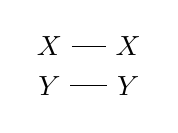
\begin{tikzpicture}
\path (0,0) node (E) {$X$}
++(1,0) node (F) {$X$}
(0,-0.5) node (F1) {$Y$}
+(1,0) node (G) {$Y$};
\draw (E) -- (F);
\draw (F1) -- (G);
\end{tikzpicture}\\
&= 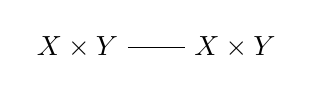
\begin{tikzpicture}
\path (0,0) node (X) {$X\times Y$}
++(2,0) node (Y) {$X\times Y$};
\draw (X) -- (Y);
\end{tikzpicture}
\end{align}

A kernel $\kernel{L}:X\kto Y\times Z$ can be written using either two parallel output wires or a single output wire, appropriately labeled:

\begin{align}
&\begin{tikzpicture}
\path (0,0) node (E) {$X$}
++ (1,0) node[kernel] (L) {$\kernel{L}$}
++ (1,0.15) node (F) {$Y$}
+(0,-0.3) node (G) {$Z$};
\draw (E) -- (L);
\draw ($(L.east) + (0,0.15)$) -- (F);
\draw ($(L.east)+ (0,-0.15)$) -- (G);
\end{tikzpicture}\\
&\equiv\\
&\begin{tikzpicture}
\path (0,0) node (E) {$X$}
++ (1,0) node[kernel] (L) {$\kernel{L}$}
++ (1.5,0) node (F) {$Y\times Z$};
\draw (E) -- (L) -- (F);
\end{tikzpicture}
\end{align}

We read diagrams from left to right (this is somewhat different to \citet{fritz_synthetic_2020,cho_disintegration_2019,fong_causal_2013} but in line with \citet{selinger_survey_2011}), and any diagram describes a set of nested products and tensor products of Markov kernels. There are a collection of special Markov kernels for which we can replace the generic ``box'' of a Markov kernel with a diagrammatic elements that are visually suggestive of what these kernels accomplish.

\subsection{Special maps}

\begin{definition}[Identity map]\label{def:ident_k}
The identity map $\kernel{I}_X:X\kto X$ defined by $(\kernle{I}_X)(A|x)= \delta_x(A)$ for all $x\in X$, $A\in\sigalg{X}$, is represented by a bare line.
\begin{align}
    \mathrm{I}_X&:=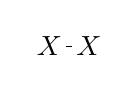
\begin{tikzpicture}[baseline={([yshift=-.5ex]current bounding box.center)}]
    \path (0,0) node (A) {$X$} ++ (0.5,0) node (B) {$X$};
    \draw (A) -- (B);
\end{tikzpicture}
\end{align}
\end{definition}

\begin{definition}[Erase map]\label{def:erase}
Given some 1-element set $\{*\}$, the erase map $\text{del}_X:X\kto \{*\}$ is defined by $(\text{del}_X)(*|x) = 1$ for all $x\in X$. It ``discards the input''. It looks like a lit fuse:
\begin{align}
    \text{del}_X&:=\begin{tikzpicture}[baseline={([yshift=-.5ex]current bounding box.center)}]
    \path (0,0) ++ (1,0) node (B) {$X$};
    \draw[-{Rays[n=8]}] (A) -- (B);
\end{tikzpicture}
\end{align}
\end{definition}

\begin{definition}[Swap map]\label{def:swap}
The swap map $\text{swap}_{X,Y}:X\times Y\kto Y\times X$ is defined by $(\text{swap}_{X,Y})(A\times B|x,y)=\delta_x(B)\delta_y(A)$ for $(x,y)\in X\times Y$, $A\in \sigalg{X}$ and $B\in \sigalg{Y}$. It swaps two inputs and is represented by crossing wires:
\begin{align}
    \text{swap}_{X,Y} &:=  
\begin{tikzpicture}[baseline={([yshift=-.5ex]current bounding box.center)}]
        \path (0,0) node (A) {} 
        + (0,-0.5) node (B) {}
        ++ (1,0) node (C) {}
        + (0,-0.5) node (D) {};
        \draw (A) to [out=0,in=180] (D) (B) to [out=0, in=180] (C);
    \end{tikzpicture}
\end{align}
\end{definition}

\begin{definition}[Copy map]\label{def:copy}
The copy map $\text{copy}_X:X\kto X\times X$ is defined by $(\text{copy}_X)(A\times B|x)=\delta_x(A)\delta_x(B)$ for all $x\in X$, $A,B\in \sigalg{X}$. It makes two identical copies of the input, and is drawn as a fork:
\begin{align}
    \text{copy}_X&:=\begin{tikzpicture}[baseline={([yshift=-.5ex]current bounding box.center)}]
    \path (0,0) node (A) {$X$} 
    ++ (0.5,0) node[copymap] (copy0) {}
    ++ (0.5,0.15) node (B) {$X$}
    + (0,-0.3) node (C) {$X$};
    \draw (A) -- (copy0) to [out=45,in=180] (B) (copy0) to [out=-45, in=180] (C);
\end{tikzpicture}
\end{align}
\end{definition}

\begin{definition}[$n$-fold copy map]
The $n$-fold copy map $\text{copy}^n_X:X\kto X^n$ is given by the recursive definition
\begin{align}
    \text{copy}^1_X &= \text{copy}_X\\
    \text{copy}^n_X &= \tikzfig{n_fold_copy} &n>1
\end{align}
\end{definition}

\paragraph{Plates}\label{pgph:plates}

In a string diagram, a plate that is annotated $i\in A$ means the tensor product of the $|A|$ elements that appear inside the plate. A wire crossing from outside a plate boundary to the inside of a plate indicates an $|A|$-fold copy map, which we indicate by placing a dot on the plate boundary. For our purposes, we do not define anything that allows wires to cross from the inside of a plate to the outside; wires must terminate within the plate.

Thus, given $\kernel{K}_i:X\kto Y$ for $i\in A$,

\begin{align}
    \bigotimes_{i\in A} \kernel{K}_i &:= \tikzfig{plate_without_copymap}
    \text{Copy}^{|A|}_X(\bigotimes_{i\in A} \kernel{K}_i) &:= \tikzfig{plate_with_copymap}
\end{align}

\subsection{Commutative comonoid axioms}

Diagrams in Markov categories satisfy the commutative comonoid axioms.

\begin{align}
    \tikzfig{ccom_lhs} = \tikzfig{ccom_rhs}\label{eq:ccom_1}
\end{align}
\begin{align}
    \tikzfig{ccom2_lhs} = \tikzfig{ccom2_mhs} = \tikzfig{ccom2_rhs}\label{eq:ccom2_del}
\end{align}
\begin{align}
    \tikzfig{ccom3_lhs} = \tikzfig{ccom3_rhs} \label{eq:ccom3_swap}
\end{align}
as well as compatibility with the monoidal structure
\begin{align}
    \tikzfig{mstruct1_lhs} &= \tikzfig{mstruct1_rhs}\\
    \tikzfig{mstruct2_lhs} &= \tikzfig{mstruct2_rhs}
\end{align}
and the naturality of \emph{del}, which means that
\begin{align}
    \tikzfig{naturality_lhs} &= \tikzfig{naturality_rhs}\label{eq:nat}
\end{align}


\subsection{Examples of using string diagrams}\label{sssec:string_diagram_manipulation}

Planar deformations along with the applications of Equations \eqref{eq:ccom_1} through to Equation \eqref{eq:nat} are almost the only rules we have for transforming one string diagram into an equivalent one. One further rule is given by Theorem \ref{th:fong_det_kerns}.

\begin{theorem}[Copy map commutes for deterministic kernels \citep{fong_causal_2013}]\label{th:fong_det_kerns}
For $\kernel{K}:X\kto Y$
\begin{align}
	\tikzfig{deterministic_copymap_commute}
\end{align}
holds iff $\kernel{K}$ is deterministic.
\end{theorem}

\subsubsection{Notation conversion}

String diagrams can always be converted into definitions involving integrals and tensor products. A number of shortcuts can help to make the translations efficiently.

For arbitrary $\kernel{K}:X\times Y\kto Z$, $\kernel{L}:W\kto Y$

\begin{align}
    \tikzfig{identity_tensor_L} &= (\kernel{I}_X\otimes \kernel{L})\kernel{K}\\
    [(\kernel{I}_X\otimes \kernel{L})\kernel{K}](A|x,w) &= \int_{Y}\int_X   \kernel{K}(A|x',y')\kernel{L}(\mathrm{d}y'|w)\delta_x(\mathrm{d}x')\\
                                           &= \int_Y  \kernel{K}(A|x,y') \kernel{L}(dy'|w)
\end{align}

That is, an identity map ``passes its input directly to the next kernel''. 

For arbitrary $\kernel{K}: X\times Y\times Y\kto Z$:

\begin{align}
 \tikzfig{identity_tensor_copy} &= (\kernel{I}_X\otimes \text{Copy}_Y)\kernel{K}\\
 [(\kernel{I}_X\otimes \text{Copy}_Y)\kernel{K}](A|x,y) &= \int_Y\int_Y \kernel{K}(A|x,y',y'') \delta_y(\mathrm{d}y')\delta_y(\mathrm{d}y'')\\
                                           &= \kernel{K}(A|x,y,y)
\end{align}

That is, the copy map ``passes along two copies of its input'' to the next kernel in the product. 

For arbitrary $\kernel{K}:X\times Y\kto Z$

\begin{align}
    \tikzfig{swap_example} &= \text{swap}_{YX} \kernel{K}\\
    (\text{swap}_{YX}\kernel{K})(A|y,x) &= \int_{X\times Y} \kernel{K}(A|x',y')\delta_y(\mathrm{d}y')\delta_x(\mathrm{d}x')\\
                                        &= \kernel{K}(A|x,y)
\end{align}

The swap map before a kernel switches the input arguments.

For arbitrary $\kernel{K}:X\kto Y\times Z$

\begin{align}
    \tikzfig{swap_example_2} &= \kernel{K}\text{swap}_{YZ}\\
    (\kernel{K}\text{swap}_{YZ})(A\times B|x) &= \int_{Y\times Z} \delta_{y}(B)\delta_{z}(A)\kernel{K}(\mathrm{d}y\times\mathrm{d}z|x)\\
    &= \int_{B\times A} \kernel{K}(\mathrm{d}y\times\mathrm{d}z|x)\\
    &= \kernel{K}(B\times A|x)
\end{align}

Given $\kernel{K}:X\kto Y$ and $\kernel{L}:Y\kto Z$:

\begin{align}
	(\kernel{K}\cprod \kernel{L})(\kernel{I}_{Y}\otimes \mathrm{del}_Z) &= \tikzfig{semidirect_K_L}\\
	 &= \tikzfig{semidirect_K_L_2} &\text{by Eq. \eqref{eq:nat}}\\
	 &= \tikzfig{semidirect_K_L_3} &\text{by Eq. \eqref{eq:ccom2_del}}
\end{align}

Thus the action of the $\text{del}$ map is to marginalise over the deleted wire. With integrals, we can write

\begin{align}
	(\kernel{K}\cprod \kernel{L})(\kernel{I}_{Y}\otimes \mathrm{del}_Z)(A\times\{*\}|x) &= \int_{Y}\int_{\{*\}}\delta_y(A)\delta_{*}(\{*\})\kernel{L}(\mathrm{d}z|y)\kernel{K}(\mathrm{d}y|x)\\
	&= \int_A \kernel{K}(\mathrm{d}y|x)\\
	&= \kernel{K}(A|x)
\end{align}

\subsubsection{Substitution}

Just like when manipulating ordinary mathematical notation, we can substitute equivalent subdiagrams in a larger diagram. That is, if we have

\begin{align}
	\tikzfig{joint_conditional} = \tikzfig{decomposed_conditional}
\end{align}

Then we can substitute the left hand side for the right hand side:

\begin{align}
	\tikzfig{joint_distribution} = \tikzfig{decomposed_joint_distribution}
\end{align}


\subsubsection{Equivalence}

We can include multiple copies of the same Markov kernel in a diagram. We can use this to show, for example, that certain conditionals are equivalent. For example, we can represent the following (see Section \ref{sec:eci} for the definition of conditional independence $\CI$)

\begin{align}
	(\RV{X}_2, \RV{Y}_2) &\CI_{\prob{P}} (\RV{Y}_1,\RV{X}_1) | \RV{H}\\
	\prob{P}^{\RV{Y}_1|\RV{X}_1\RV{H}} &= \prob{P}^{\RV{Y}_2|\RV{X}_2\RV{H}}
\end{align}

with the following diagram equation:
\begin{align}
	\prob{P}^{\RV{X_{\{1,2\}}\RV{Y}_{\{1,2\}}|\RV{H}}} &= \tikzfig{y_indep_example_joint}\label{eq:defn_indep_w_diagram}
\end{align}
Note that in this diagram, we have implicitly
\begin{align}
	\prob{P}^{\RV{X}_1|\RV{H}} &= \kernel{K}_1\\
	\prob{P}^{\RV{X}_2|\RV{H}} &= \kernel{K}_2\\
	\prob{P}^{\RV{Y}_1|\RV{X}_1\RV{H}} &= \prob{P}^{\RV{Y}_2|\RV{X}_2\RV{H}}\\
	&= \kernel{L}
\end{align}
if a kernel in a diagram is equal to $\prob{P}^{\RV{W}|\RV{U}}$ we will typically label it explicitly as such for clarity, but as in Eq. \eqref{eq:defn_indep_w_diagram}, it is not strictly necessary to do so.

\subsubsection{Surgery}

We can also use string diagrams to compactly define ``surgery'' operations that take a probability distribution and return a probability distribution with a subset of the Markov kernels transformed. A standard definition of hard interventions in causal models is to separately define a transformation of the probability distribution takes a directed acyclic graph

\begin{align}
	\mathcal{G} = \tikzfig{simple_dag}
\end{align}

and defines a transformation of the joint probability distribution with respect to this graph (see Definition \ref{def:CBN} for a more precise explanation of interventions):

\begin{align}
	\prob{P}^{\RV{Y}|\mathrm{do}(\RV{X}=x)} = \sum_{z\in Z} \prob{P}^{\RV{Y}|\RV{X}\RV{Z}}(\cdot|x,z)
\end{align}

and separately defines a transformed graph $\mathcal{G}_{\overline{\RV{X}}}$ associated with the operation

\begin{align}
	\mathcal{G}_{\overline{X}} = \tikzfig{simple_dag_cut}
\end{align}

\citet{jacobs_causal_2019} defines the ``cut'' operation on string diagrams which subsumes both the graphical and probabilistic definition of an intervention. It involves (in this example) replacing the Markov kernel associated with $\prob{P}^{\RV{X}|\RV{Z}}$ with the markov kernel $\kernel{K}_x:= *\mapsto \delta_x$.

\begin{align}
	\mathrm{cut}(\tikzfig{simple_dag_as_string}) = \tikzfig{simple_dag_as_string_cut}
\end{align}


\section{Probability Sets and Decision Models}\label{sec:probability_sets}

A probability set is a set of probability measures. This section establishes a number of useful properties of conditional probability with respect to probability sets. Unlike conditional probability with respect to a probability space, conditional probabilities don't always exist for probability sets. Where they do, however, they are almost surely unique and we can marginalise and disintegrate them to obtain other conditional probabilities with respect to the same probability set.

First, we define a \emph{decision model} as a triple of a probability set along with an indexing \emph{option set} and the common sample space. We could also consider a decision model to be a function $C\kto \Omega$, where we do not distinguish options options $\alpha,\alpha'\in C$ that induce the same probability distributions (i.e. $\prob{P}_\alpha=\prob{P}_{\alpha'}$).

\begin{definition}[Decision model]\label{def:dec_model}
A decision model is a triple $(\prob{P}_\cdot, (\Omega,\sigalg{F}), (C,\sigalg{C}))$ where $\prob{P}_\cdot:C\kto \Omega$ is a Markov kernel, $(\Omega,\sigalg{F})$ is the shared sample space and $C$ is the option set.
\end{definition}

Decision models induce sets of probability distributions: for some $A\subset C$, $\prob{P}_A:=\{\prob{P}_\alpha|\alpha\in A\}$ is the set of probability distributions induced by $A$.

\begin{definition}[Probability set]\label{def:prob_set}
A probability set $\prob{P}_C$ on $(\Omega,\sigalg{F})$ is a collection of probability measures on $(\Omega,\sigalg{F})$. In other words it is a subset of $\mathscr{P}(\Delta(\Omega))$, where $\mathscr{P}$ indicates the power set.
\end{definition}

Given a probability set $\prob{P}_C$, we define marginal and conditional probabilities as probability measures and Markov kernels that satisfy Definitions \ref{def:pushforward} and \ref{def:disint} respectively for \emph{all} base measures in $\prob{P}_C$. There are generally multiple Markov kernels that satisfy the properties of a conditional probability with respect to a probability set, and this definition ensures that marginal and conditional probabilities are ``almost surely'' unique (Definition \ref{def:asequal}) with respect to probability sets.

\begin{definition}[Marginal probability with respect to a probability set]
Given a sample space $(\Omega,\sigalg{F})$, a variable $\RV{X}:\Omega\to X$ and a probability set $\prob{P}_C$, the marginal distribution $\prob{P}_C^{\RV{X}}=\prob{P}_\alpha^{\RV{X}}$ for any $\prob{P}_\alpha\in\prob{P}_C$ if a distribution satisfying this condition exists. Otherwise, it is undefined.
\end{definition}

\begin{definition}[Uniform conditional distribution]\label{def:cprob_pset}
Given a sample space $(\Omega,\sigalg{F})$, variables $\RV{X}:\Omega\to X$ and $\RV{Y}:\Omega\to Y$ and a probability set $\prob{P}_C$, a uniform conditional distribution $\prob{P}_C^{\RV{Y}|\RV{X}}$ is any Markov kernel $X\kto Y$ such that $\prob{P}_C^{\RV{Y}|\RV{X}}$ is an $\RV{Y}|\RV{X}$ conditional probability of $\prob{P}_\alpha$ for all $\prob{P}_\alpha\in \prob{P}_C$. If no such Markov kernel exists, $\prob{P}_C^{\RV{Y}|\RV{X}}$ is undefined.
\end{definition}

Given a conditional distribution $\mu^{\RV{ZY}|\RV{X}}$ we can define a higher order conditional $\mu^{\RV{Z}|(\RV{Y}|\RV{X})}$, which is a version of $\mu^{\RV{Z}|\RV{XY}}$. This is useful because uniform conditionals don't always exist, but we can use higher order conditionals to show that if a probability set $\prob{P}_C$ has a uniform conditional $\prob{P}_C^{\RV{ZY}|\RV{X}}$ then it also has a uniform conditional $\prob{P}_C^{\RV{Z}|\RV{XY}}$ (Theorems \ref{th:ho_cond_psets} and \ref{th:higher_order_conditionals}). Given $\mu^{\RV{XY}|\RV{Z}}$ and $\RV{X}:\Omega\to X$, $\RV{Y}:\Omega\to Y$ standard measurable, it has recently been proven that a higher order conditional $\mu^{\RV{Z}|(\RV{Y}|\RV{X})}$ exists \citet{bogachev_kantorovich_2020}, Theorem 3.5.

\begin{definition}[Higher order conditionals]
Given a probability space $(\mu,\Omega,\sigalg{F})$ and variables $\RV{X}:\Omega\to X$, $\RV{Y}:\Omega\to Y$ and $\RV{Z}:\Omega\to Z$, a higher order conditional $\mu^{\RV{Z}|(\RV{Y}|\RV{X})}:X\times Y\to Z$ is any Markov kernel such that, for some $\mu^{\RV{Y}|\RV{X}}$, 
\begin{align}
    \mu^{\RV{ZY}|\RV{X}}(B\times C|x) &=\int_B \mu^{\RV{Z}|(\RV{Y}|\RV{X})}(C|x,y)\mu^{\RV{Y}|\RV{X}}(dy|x)\\ 
    &\iff\\
    \mu^{\RV{ZY}|\RV{X}} &= \tikzfig{disintegration_existence}\label{eq:disint_def}
\end{align}
\end{definition}

\begin{definition}[Uniform higher order conditional]\label{def:ho_cprob_pset}
Given a sample space $(\Omega,\sigalg{F})$, variables $\RV{X}:\Omega\to X$, $\RV{Y}:\Omega\to Y$ and $\RV{Z}:\Omega\to Z$ and a probability set $\prob{P}_C$, if $\prob{P}_C^{\RV{ZY}|\RV{X}}$ exists then a uniform higher order conditional $\prob{P}_C^{\RV{Z}|(\RV{Y}|\RV{X})}$ is any Markov kernel $X\times Y\kto Z$ that is a higher order conditional of some version of $\prob{P}_C^{\RV{ZY}|\RV{X}}$. If no $\prob{P}_C^{\RV{ZY}|\RV{X}}$ exists, $\prob{P}_C^{\RV{Z}|(\RV{Y}|\RV{X})}$ is undefined.
\end{definition}

\begin{definition}[Almost sure equality]
Two Markov kernels $\kernel{K}:X\kto Y$ and $\kernel{L}:X\kto Y$ are $\prob{P}_C,\RV{X},\RV{Y}$-almost surely equal if for all $A\in\sigalg{X}$, $B\in \sigalg{Y}$, $\alpha\in C$
\begin{align}
    \int_A \kernel{K}(B|x)\prob{P}_\alpha^{\RV{X}}(\mathrm{d}x) = \int_A\kernel{L}(B|x)\prob{P}_\alpha^{\RV{X}}(\mathrm{d}x)
\end{align}
we write this as $\kernel{K}\overset{\prob{P}_C}{\cong}\kernel{L}$, as the variables $\RV{X}$ and $\RV{Y}$ are clear from the context.
\end{definition}

Equivalently, $\kernel{K}$ and $\kernel{L}$ are almost surely equal if the set $C:\{x|\exists B\in\sigalg{Y}:\kernel{K}(B|x)\neq\kernel{L}(B|x)\}$ has measure 0 with respect to $\prob{P}_\alpha^{\RV{X}}$ for all $\alpha\in C$.

\subsection{Almost sure equality}

Two Markov kernels are almost surely equal with respect to a probability set $\prob{P}_C$ if the semidirect product $\odot$ of all marginal probabilities of $\prob{P}_\alpha^\RV{X}$ with each Markov kernel is identical.

\begin{definition}[Almost sure equality]\label{def:asequal}
Two Markov kernels $\kernel{K}:X\kto Y$ and $\kernel{L}:X\kto Y$ are almost surely equal $\overset{\prob{P}_C}{\cong}$ with respect to a probability set $\prob{P}_C$ and variable $\RV{X}:\Omega\to X$ if for all $\prob{P}_\alpha \in \prob{P}_C$,
\begin{align}
    \prob{P}^{\RV{X}}_\alpha\odot \kernel{K}=\prob{P}^{\RV{X}}_\alpha\odot \kernel{L}
\end{align}
\end{definition}

\begin{lemma}[Uniform conditional distributions are almost surely equal]
If $\kernel{K}:X\kto Y$ and $\kernel{L}:X\kto Y$ are both versions of $\prob{P}_C^{\RV{Y}|\RV{X}}$ then $\kernel{K}\overset{\prob{P}_C}{\cong}\kernel{L}$
\end{lemma}

\begin{proof}
For all $\prob{P}_\alpha \in \prob{P}_C$
\begin{align}
    \prob{P}^{\RV{X}}_\alpha\odot \kernel{K} &= \prob{P}^{\RV{XY}}_\alpha\\
    &= \prob{P}^{\RV{X}}_\alpha\odot \kernel{L}
\end{align}
\end{proof}

\begin{lemma}[Substitution of almost surely equal Markov kernels]\label{lem:sub_asequal}
Given $\prob{P}_C$, if $\kernel{K}:X\times Y \kto Z$ and $\kernel{L}:X\times Y \kto Z$ are almost surely equal $\kernel{K}\overset{\prob{P}_C}{\cong}\kernel{L}$, then for any $\prob{P}_\alpha\in \prob{P}_C$
\begin{align}
    \prob{P}_\alpha^{\RV{Y}|\RV{X}}\odot \kernel{K} &\overset{\prob{P}_C}{\cong} \prob{P}_\alpha^{\RV{Y}|\RV{X}}\odot \kernel{L}
\end{align}
\end{lemma}

\begin{proof}
For any $\prob{P}_\alpha\in\prob{P}_C$
\begin{align}
    \prob{P}_\alpha^{\RV{XY}}\odot \kernel{K} &\overset{\prob{P}_C}{\cong} (\prob{P}_\alpha^{\RV{X}}\odot \prob{P}_C^{\RV{Y}|\RV{X}})\odot \kernel{K}\\
                                              &\overset{\prob{P}_C}{\cong} \prob{P}_\alpha^{\RV{X}}\odot (\prob{P}_C^{\RV{Y}|\RV{X}}\odot \kernel{K})\\
                                              &\overset{\prob{P}_C}{\cong} \prob{P}_\alpha^{\RV{X}}\odot (\prob{P}_C^{\RV{Y}|\RV{X}}\odot \kernel{L})
\end{align}
\end{proof}

\begin{theorem}[Semidirect product of uniform conditional distributions is a joint uniform conditional distribution]\label{lem:joint_conditional}
Given a probability set $\prob{P}_C$ on $(\Omega,\sigalg{F})$, variables $\RV{X}:\Omega\to X$, $\RV{Y}:\Omega\to Y$ and uniform conditional distributions $\prob{P}_C^{\RV{Y}|\RV{X}}$ and $\prob{P}_C^{\RV{Z}|\RV{XY}}$, then $\prob{P}_C^{\RV{YZ}|\RV{X}}$ exists and is equal to
\begin{align}
    \prob{P}_C^{\RV{YZ}|\RV{X}} &\overset{\prob{P}_C}{\cong} \prob{P}_C^{\RV{Y}|\RV{X}}\odot \prob{P}_C^{\RV{Z}|\RV{XY}}
\end{align}
\end{theorem}

\begin{proof}
By definition, for any $\prob{P}_\alpha\in \prob{P}_C$
\begin{align}
    \prob{P}_\alpha^{\RV{XYZ}} &= \prob{P}_\alpha^{\RV{X}}\odot \prob{P}_\alpha^{\RV{YZ}|\RV{X}}\\
                               &= \prob{P}_\alpha^{\RV{X}}\odot(\prob{P}_\alpha^{\RV{Y}|\RV{X}}\odot \prob{P}_\alpha^{\RV{Z}|\RV{YX}})\\
                               &= \prob{P}_\alpha^{\RV{X}}\odot(\prob{P}_C^{\RV{Y}|\RV{X}}\odot \prob{P}_C^{\RV{Z}|\RV{YX}})
\end{align}
\end{proof}

\subsection{Existence of conditional distributions}

It is known that conditional distributions do not exist in general for probability measures defined on arbitrary measurable sets. However, the requirement that the sets are \emph{standard measurable} is sufficient for the existence of conditional distributions. We also further show that, given a borel measurable map to standard measurable probability distributions, what we call ``higher order conditionals'' also exist.

\begin{lemma}[Conditional pushforward]\label{th:recurs_pushf}
Suppose we have a sample space $(\Omega,\sigalg{F})$, variables $\RV{X}:\Omega\to X$ and $\RV{Y}:\Omega\to Y$, $\RV{Z}:\Omega\to Z$ and a probability set $\prob{P}_C$ with conditional $\prob{P}_C^{\RV{Y}|\RV{X}}$ such that $\RV{Z}=f\circ \RV{Y}$ for some $f:Y\to Z$. Then there exists a conditional probability $\prob{P}_C^{\RV{Z}|\RV{X}}=\prob{P}_C^{\RV{Y}|\RV{X}}\kernel{F}_{f}$.
\end{lemma}

\begin{proof}
Note that $(\RV{X},\RV{Z})=(\mathrm{Id}_X\otimes f)\circ (\RV{X},\RV{Y})$. Thus, by Lemma \ref{lem:pushf_kprod}, for any $\prob{P}_\alpha\in \prob{P}_C$

\begin{align}
    \prob{P}_\alpha^{\RV{XZ}} = \prob{P}_\alpha^{\RV{XY}}\kernel{F}_{\mathrm{Id}_X\otimes f}
\end{align}

Note also that for all $A\in\sigalg{X}$, $B\in \sigalg{Z}$, $x\in X$, $y\in Y$:

\begin{align}
\prob{F}_{\mathrm{Id}}_X\otimes f}(A\times B|x,y)&=\delta_x(A)\delta_{f(y)}(B)\\
&= \prob{F}_{\mathrm{Id}}_X} (A|x)\otimes \prob{F}_f(B|y)\\
\implies \prob{F}_{\mathrm{Id}}_X\otimes f} &= \prob{F}_{\mathrm{Id}}_X} \otimes \prob{F}_f
\end{align}

Thus

\begin{align}
    \prob{P}_\alpha^{\RV{XZ}} &= (\prob{P}_\alpha^{\RV{X}}\odot \prob{P}_C^{\RV{Y}|\RV{X}})\kernel{F}_{\mathrm{Id}_X}\otimes \kernel{F}_f\\
    &= \tikzfig{conditional_pushforward}
\end{align}

Which implies $\prob{P}_C^{\RV{Y}|\RV{X}}\kernel{F}_{f}$ is a version of $\prob{P}_{\alpha}^{\RV{Z}|\RV{X}}$. Because this holds for all $\alpha$, it is therefore also a version of $\prob{P}_C^{\RV{Z}|\RV{X}}$.
\end{proof}

The following theorem is a standard result in many probability texts. In this work, the measurable spaces considered will all be standard measurable and so Theorem \ref{th:reg_cond} always applies. We will simply assume that conditional probabilities exist, and avoid referencing this theorem every time.

\begin{theorem}[Existence of regular conditionals]\label{th:reg_cond}
Suppose we have a sample space $(\Omega,\sigalg{F})$, variables $\RV{X}:\Omega\to X$ and $\RV{Y}:\Omega\to Y$ with $Y$ standard measurable and a probability model $\prob{P}_{\alpha}$ on $(\Omega,\sigalg{F})$. Then there exists a conditional $\prob{P}_\alpha^{\RV{Y}|\RV{X}}$.
\end{theorem}

\begin{proof}
\citet[Theorem 2.18]{cinlar_probability_2011}
\end{proof}

The following theorem was proved by \citet{bogachev_kantorovich_2020}.

\begin{theorem}\label{th:bogachev}
Given a Borel measurable map $\kernel{M}:X\kto Y\times Z$ let $\Pi_Y:Y\times Z\to Y$ be the projection onto $Y$. Then there exists a Borel measurable map $\kernel{N}:X\times Y\kto Y\times Z$ such that 
\begin{align}
    \kernel{N}(\Pi_Y^{-1}(y)|x,y) &= 1\label{eq:proper}\\
    \kernel{M}(\RV{Y}^{-1}(A)\cap B|x) &= \int_A \kernel{N}(B|x,y) \kernel{M}\kernel{F}_{\Pi_Y}(dy|x)&\forall A\in \sigalg{Y},B\in\sigalg{Y\times Z}\label{eq:conditional1}
\end{align}
\end{theorem}

\begin{proof}
 \citet[Theorem 3.5]{bogachev_kantorovich_2020}
\end{proof}

The following corollary implies that, given a uniform conditional, higher order conditionals can generically be found for probability sets.

\begin{corollary}[Existence of higher order conditionals with respect to probability sets]\label{th:ho_cond_psets}
Take a sample space $(\Omega,\sigalg{F})$, variables $\RV{X}:\Omega\to X$ and $\RV{Y}:\Omega\to Y$, $\RV{Z}:\Omega\to Z$ and a probability set $\prob{P}_C$ with uniform conditional distribution $\prob{P}_C^{\RV{YZ}|\RV{X}}$, and $Y$ and $Z$ standard measurable. Then there exists a higher order uniform conditional $\prob{P}_C^{\RV{Z}|(\RV{Y}|\RV{X})}$.
\end{corollary}

\begin{proof}
Take $\prob{P}_C^{\RV{YZ}|\RV{X}}$ to be the Borel measurable map $\kernel{M}$ from Theorem \ref{th:bogachev}, and note that $\Pi_Y\circ (\RV{Y},\RV{Z})=\RV{Y}$. Then equation \eqref{eq:conditional1} implies for all $A\in \sigalg{Y},B\in\sigalg{Y\times Z}$ there is some $\kernel{N}$ such that

\begin{align}
    \prob{P}_C^{\RV{YZ}|\RV{X}}(\RV{Y}^{-1}(A)\cap B|x) &= \int_A \kernel{N}(B|x,y) \prob{P}_C^{\RV{YZ}|\RV{X}}\kernel{F}_{\Pi_Y}(dy|x)\\
    &=\int_A \kernel{N}(B|x,y) \prob{P}_C^{\RV{Y}|\RV{X}}(dy|x)\label{eq:rec_push}
\end{align}
where Equation \eqref{eq:rec_push} follows from Lemma \ref{th:recurs_pushf}.

Then, for any $\prob{P}_\alpha\in\prob{P}_C$
\begin{align}
    \prob{P}_C^{\RV{YZ}|\RV{X}}(\RV{Y}^{-1}(A)\cap B|x) &= \int_A \kernel{N}(B|x,y) \prob{P}_{\alpha}^{\RV{Y}|\RV{X}}(dy|x)
\end{align}
which implies $\kernel{N}$ is a version of $\prob{P}_C^{\RV{YZ}|(\RV{Y}|\RV{X})}$. By Lemma \ref{th:recurs_pushf}, $\kernel{N}\kernel{F}_{\Pi_Y}$ is a version of $\prob{P}_C^{\RV{Z}|(\RV{Y}|\RV{X})}$.
\end{proof}

\subsection{Extended conditional independence}\label{sec:eci}

Just like we defined uniform conditional probability as a version of ``conditional probability'' appropriate for probability sets, we need some version of ``conditional independence'' for probability sets. One such has already been given in some detail: it is the idea of \emph{extended conditional independence} defined in \citet{constantinou_extended_2017}.

We will first define regular conditional independence. We define it in terms of a having a conditional that ``ignores one of its inputs'', which, provided conditional probabilities exists, is equivalent to other common definitions (Theorem \ref{th:cho_ci_equiv}).

\begin{definition}[Conditional independence]\label{def:ci}
For a \emph{probability model} $\model{P}_{\alpha}$ and variables $\RV{W},\RV{X},\RV{Y}$, we say $\RV{Y}$ is conditionally independent of $\RV{X}$ given $\RV{W}$, written $\RV{Y}\CI_{\model{P}_{\alpha}}\RV{X}|\RV{W}$, if
\begin{align}
    \prob{P}_\alpha^{\RV{Y}|\RV{WX}} &\overset{\prob{P}_\alpha}{\cong} \tikzfig{cond_indep_erase}\\
    \iff
    \prob{P}_\alpha^{\RV{Y}|\RV{WX}}(A|w,x) &\overset{\prob{P}_\alpha}{\cong} \prob{K}(A|w)&\forall A\in \sigalg{Y}, \text{ some }\kernel{K}:W\kto Y
\end{align}
\end{definition}

Conditional independence can equivalently be stated in terms of the existence of a conditional probability that ``ignores'' one of its inputs.

\begin{theorem}\label{th:cho_ci_equiv}
Given standard measurable $(\Omega,\sigalg{F})$, a probability model $\prob{P}_\alpha$ and variables $\RV{W}:\Omega\to W$, $\RV{X}:\Omega\to X$, $\RV{Y}:\Omega\to Y$, $\RV{Y}\CI_{\prob{P}}\RV{X}|\RV{W}$ if and only if there exists some version of $\prob{P}_\alpha^{\RV{Y}|\RV{WX}}$ and $\kernel{K}:W\kto Y$ such that
\begin{align}
    \prob{P}_\alpha^{\RV{XY}|\RV{W}} &\overset{\prob{P}}{\cong} \tikzfig{cond_indep_product}\\
    \iff
    \prob{P}_\alpha^{\RV{XY}|\RV{W}}(A\times B|w) &\overset{\prob{P}_\alpha}{\cong} \prob{P}_\alpha^{\RV{X}|\RV{W}}(A|w)\prob{P}_\alpha^{\RV{Y}|\RV{W}}(B|w)&\forall A\in \sigalg{X}, B\in \sigalg{Y}
\end{align}
\end{theorem}

\begin{proof}
See \citet{cho_disintegration_2019}.
\end{proof}

Extended conditional independence as introduced by \citet{constantinou_extended_2017} is defined in terms of ``nonstochastic variables'' on the option set C. A nonstochastic variable is essentially a variable defined on $C$ rather than on the sample space $\Omega$

\begin{definition}[Nonstochastic variable]\label{def:nonstoc_var}
Given a sample space $(\Omega,\sigalg{F})$, a choice set $(C,\sigalg{C})$, a codomain $(X,\sigalg{X})$ and a probability set $\prob{P}_C$, a nonstochastic variable is a measurable function $\phi:C\to X$.
\end{definition}

In particular, we want to consider \emph{complementary} nonstochastic variable - that is, pairs of nonstochastic variables $\phi$ and $\xi$ such that the sequence $(\phi,\xi)$ is invertible. For example, if $\phi:=\mathrm{Id}_C$, then $\phi$ and $*$ are a pair of complementary variables.

\begin{definition}[Complementary nonstochastic variables]\label{def:comp_var}
A pair of nonstochastic variables $\phi$ and $\xi$ are complementary if $(\phi,\xi)$ is invertible.
\end{definition}

\begin{notation}
The letters $\phi$ and $\xi$ are used to represent complementary nonstochastic variables.
\end{notation}

Unlike \citet{constantinou_extended_2017}, we limit ourselves to a definition of extended conditional independence where regular uniform conditional probabilities exist. Our definition is otherwise identical.

\begin{definition}[Extended conditional independence]\label{def:eci_orig}
Given a probability set $\prob{P}_C$, variables $\RV{X}$, $\RV{Y}$ and $\RV{Z}$ and complementary nonstochastic variables $\phi$ and $\xi$, the extended conditional independence $\RV{Y}\CI^e_{\prob{P}_C} \RV{X} \phi|\RV{Z} \xi$ holds if for each $a\in \xi(C)$, $\prob{P}_{\xi^{-1}(a)}^{\RV{Y}|\RV{XZ}}$ and $\prob{P}_{\xi^{-1}(a)}^{\RV{Y}|\RV{X}}$ exist and
\begin{align}
    \prob{P}_{\xi^{-1}(a)}^{\RV{Y}|\RV{XZ}} &\overset{\prob{P}_{\xi^{-1}(a)}}{\cong} \tikzfig{eci_def}\\
    &\iff\\
    \prob{P}_{\xi^{-1}(a)}^{\RV{Y}|\RV{XZ}}(A|x,z) &\overset{\prob{P}_{\xi^{-1}(a)}}{\cong} \prob{P}_{\xi^{-1}(a)}^{\RV{Y}|\RV{Z}}(A|z)&\forall A\in \sigalg{Y},(x,z)\in X\times Z\label{eq:eci}
\end{align}
\end{definition}

Very often, we consider a particular kind of extended conditional independence that does not explicitly make use of nonstochastic variables. We call this \emph{uniform conditional independence}.

\begin{definition}[Uniform conditional independence]\label{def:eci}
Given a probability set $\prob{P}_C$ and variables $\RV{X}$, $\RV{Y}$ and $\RV{Z}$, the uniform conditional independence $\RV{Y}\CI^e_{\prob{P}_C} (\RV{X}, \mathrm{Id}_C)|\RV{Z}$ holds if $\prob{P}_C^{\RV{Y}|\RV{XZ}}$ and $\prob{P}_C^{\RV{Y}|\RV{X}}$ exist and
\begin{align}
    \prob{P}_C^{\RV{Y}|\RV{XZ}} &\overset{\prob{P}_C}{\cong} \tikzfig{eci_def}\\
    &\iff\\
    \prob{P}_C^{\RV{Y}|\RV{XZ}}(A|x,z) &\overset{\prob{P}_C}{\cong} \prob{P}_C^{\RV{Y}|\RV{Z}}(A|z)&\forall A\in \sigalg{Y},(x,z)\in X\times Z\label{eq:uci}
\end{align}
\end{definition}

For countable sets $C$ (which, recall, is an assumption we generally accept), as shown by \citet{constantinou_extended_2017} we can reason with collections of extended conditional independence statements as if they were regular conditional independence statements, with the provision that a complementary pair of nonstochastic variables must appear either side of the ``|'' symbol. 

\begin{enumerate}
    \item Symmetry: $\RV{X}\CI_{\prob{P}_C}^e \RV{Y}|(\RV{Z}, \mathrm{Id}_C)$ iff $\RV{Y}\CI_{\prob{P}_C}^e \RV{X}|(\RV{Z}, \mathrm{Id}_C)$
    \item $\RV{X}\CI_{\prob{P}_C}^e \RV{Y} C| \RV{Y} C$
    \item Decomposition: $\RV{X}\CI_{\prob{P}_C}^e \RV{Y} \phi|\RV{W}\xi$ and $\RV{Z}\varlessthan\RV{Y}$ implies $\RV{X}\CI_{\prob{P}_C}^e\RV{Z}\phi|\RV{W}\xi$
    \item Weak union:
    \begin{enumerate}
     	\item $\RV{X}\CI_{\prob{P}_C}^e \RV{Y} \phi|\RV{W}\xi$ and $\RV{Z}\varlessthan \RV{Y}$ implies $\RV{X}\CI_{\prob{P}_C}^e\RV{Y}\phi|(\RV{Z},\RV{W})\xi$
     	\item $\RV{X}\CI_{\prob{P}_C}^e \RV{Y} \phi|\RV{W}\xi$ and $\lambda\varlessthan \phi$ implies $\RV{X}\CI_{\prob{P}_C}^e\RV{Y}\phi|(\RV{Z},\RV{W})(\xi,\lambda)$
     \end{enumerate} 
    \item Contraction: $\RV{X}\CI_{\prob{P}_C}^e\RV{Z}\phi|\RV{W}\xi$ and $\RV{X}\CI_{\prob{P}_C}^e\RV{Y}\phi|(\RV{Z},\RV{W})\xi$ implies $\RV{X}\CI_{\prob{P}_C}^e(\RV{Y},\RV{Z})\phi|\RV{W}\xi$
\end{enumerate} 

The following forms of these properties are often used here:

\begin{enumerate}
    \item Symmetry: $\RV{X}\CI_{\prob{P}_C}^e (\RV{Y}, \mathrm{Id}_C)|(\RV{Z}, \mathrm{Id}_C)$ iff $\RV{Y}\CI_{\prob{P}} (\RV{X}, \mathrm{Id}_C)|\RV{Z}$
    \item Decomposition: $\RV{X}\CI_{\prob{P}_C}^e (\RV{Y},\RV{Z}, \mathrm{Id}_C)|\RV{W}$ implies $\RV{X}\CI_{\prob{P}}\RV{Y}C|\RV{W}$ and $\RV{X}\CI_{\prob{P}}(\RV{Z},\mathrm{id}_C)|\RV{W}$
    \item Weak union: $\RV{X}\CI_{\prob{P}_C}^e(\RV{Y},\RV{Z},\mathrm{Id}_C)|\RV{W}$ implies $\RV{X}\CI_{\prob{P}_C}^e(\RV{Y},\mathrm{Id}_C)|(\RV{Z},\RV{W})$
    \item Contraction: $\RV{X}\CI_{\prob{P}_C}^e(\RV{Z},\mathrm{Id}_C)|\RV{W}$ and $\RV{X}\CI_{\prob{P}_C}^e(\RV{Y},\mathrm{Id}_C)|(\RV{Z},\RV{W})$ implies $\RV{X}\CI_{\prob{P}_C}^e(\RV{Y},\RV{Z},\mathrm{Id}_C)|\RV{W}$
\end{enumerate}

Conditional independence is sometimes given in terms of a factorisation of the joint conditional distribution (or joint conditional expectations). Theorem \ref{th:uci_rep} shows that the definition given here is equivalent to the definition given in terms of factorisation.

\begin{theorem}[Uniform conditional independence representation]\label{th:uci_rep}
Given a probability set $\prob{P}_C$ with a uniform conditional probability $\prob{P}^{\RV{XY}|\RV{Z}}_C$,
\begin{align}
    \prob{P}^{\RV{XY}|\RV{Z}}_C &\overset{\prob{P}_C}{\cong} \tikzfig{eci_rep}\\
    &\iff\\
    \prob{P}^{\RV{XY}|\RV{Z}}_C(A\times B|z) &\overset{\prob{P}_C}{\cong} \prob{P}_C^{\RV{X}|\RV{Z}}(A|z)\prob{P}_C^{\RV{Y}|\RV{Z}}(B|z)&\forall A\in \sigalg{X},B\in \sigalg{Y},z\in Z
\end{align}
if and only if $\RV{Y}\CI_{\prob{P}_C}^e (\RV{X},\mathrm{Id}_C)|\RV{Z}$
\end{theorem}

\begin{proof}
If:
By Theorem \ref{th:higher_order_conditionals}
\begin{align}
    \prob{P}^{\RV{XY}|\RV{Z}}_C &= \tikzfig{eci_rep_1}\\
    &\overset{\prob{P}_C}{\cong} \tikzfig{eci_rep_2}\\
    &= \tikzfig{eci_rep}
\end{align}
Only if:
Suppose
\begin{align}
    \prob{P}^{\RV{XY}|\RV{Z}}_C &\overset{\prob{P}_C}{\cong} \tikzfig{eci_rep}
\end{align}
and suppose for some $\alpha\in C$, $A\times C\in \sigalg{X}\otimes\sigalg{Z}$, $B\in \sigalg{Y}$ $\prob{P}_\alpha^{\RV{XZ}}(A\times C)>0$ and
\begin{align}
    \prob{P}_C^{\RV{Y}|\RV{XZ}}(B|x,z) &> \prob{P}_C^{\RV{Y}|\RV{Z}}(B|z)& \forall (x,z)\in A\times C \label{eq:assume_ieq}
\end{align}
then
\begin{align}
    \prob{P}_\alpha^{\RV{XYZ}}(A\times B\times C) &= \int_{A\times C} \prob{P}_C^{\RV{Y}|\RV{XZ}}(B|x,z)\prob{P}_C^{\RV{X}|\RV{Z}}(\mathrm{dx}|z)\prob{P}_\alpha^{\RV{Z}}(\mathrm{dz})\\
    &> \int_{A\times C} \prob{P}_C^{\RV{Y}|\RV{Z}}(B|z)\prob{P}_C^{\RV{X}|\RV{Z}}(\mathrm{dx}|z)\prob{P}_\alpha^{\RV{Z}}(\mathrm{dz})\\
    &= \int_{C} \prob{P}_C^{\RV{XY}|\RV{Z}}(A\times B|z)\prob{P}_\alpha^{\RV{Z}}(\mathrm{dz})\\
    &= \prob{P}_\alpha^{\RV{XYZ}}(A\times B\times C)
\end{align}
a contradiction. An analogous argument follows if we replace ``$>$'' with ``$<$'' in Eq. \eqref{eq:assume_ieq}.
\end{proof}


\section{Maximal probability sets and valid conditionals}\label{sec:validity}

So far, we have been implicitly supposing that we first set up a non-empty probability set and from that set we may sometimes derive conditional probabilities, extended conditional independences and so forth. However, sometimes we want to work backwards: start with a collection of conditional probabilities, and work with the probability set implicitly defined by this collection. This is similar to the case in which we specify how some system works by specifying, based on a priori knowledge, a set of equations that govern it. A sanity check on proposing such a set of equations is to check whether they admit any solutions, and (possibly) to check how large the set of solutions they admit is.

Similarly, proposing a collection of condiitonal probabilities may similarly be compatible with a large set of base probability distributions, a unique probability distribution or no probability distributions at all. \emph{Validity} is a sufficient (but not necessary) condition to ensure that certain collections of conditional probabilities yield a non-empty set of compatible distributions.

A particular example of specifying conditional probabilities a priori is given by Causal Bayesian Networks (see \ref{def:CBN} for more details on this kind of model). The collection of operations of the form ``$\mathrm{do}(\RV{X}=x)$'' force the conditional distribution of $\RV{X}$ given its parents to a particular value. Specifically:
\begin{align}
	\prob{P}_{\mathrm{do}_\RV{X},x}^{\RV{Y}|\mathrm{Pa}(\RV{Y})} &= \begin{cases}
	\prob{P}_{\mathrm{obs}}^{\RV{Y}|\mathrm{Pa}(\RV{Y})}&\RV{Y}\text{ is a causal variable and not equal to }\RV{X}\\
	\delta_x & \RV{Y}=\RV{X}
	\end{cases}
\end{align}

Given a causal Bayesian network with the graph $\RV{Y}\rightarrow \RV{X}$ and some observational probability distribution $\prob{P}_{\mathrm{obs}}^{\RV{XY}}\in\Delta(X\times Y)$, we conclude that $\prob{P}_{\mathrm{do}_\RV{X},x}^{\RV{X}|\RV{Y}}=\text{del}_Y \delta_x$. Suppose, however, we had $\RV{X}=\RV{Y}$ -- i.e. $\RV{X}$ and $\RV{Y}$ are actually two different labels for the same variable. Then there would be no distribution $\prob{Q}$ in $\Delta(X\times Y)$ with $\prob{Q}^{\RV{X}|\RV{Y}}=\text{del}_Y \delta_x$.

The key result of this section is: probability sets defined by collections of recursive valid conditionals and distributions are nonempty. While we suspect this condition is often satisfied by causal models in practice, we offer one example in the literature where it apparently is not. The problem of whether a probability set is valid is analogous to the problem of whether a probability distribution satisfying a collection of constraints exists discussed in \citet{vorobev_consistent_1962}. As that work shows, there are many questions of this nature that can be asked and that are not addressed by the criterion of validity.

In functional causal models, we have the notions of \emph{global compatibility} from \citet{forre_causal_2020} and \emph{unique solvability} in \citet{bongers_theoretical_2016}. These are more general than validity; they are not just sufficient but also necessary for the existence of a solution. In addition, we note that the intervention operation discussed in \citet{forre_causal_2020} preserves global compatibility, unlike the acyclic notion of intervention discussed above.

\begin{definition}[Valid distribution]\label{def:valid_dist}
Given $(\Omega,\sigalg{F})$ and a variable $\RV{X}:\Omega\to X$, an $\RV{X}$-valid probability distribution is any probability measure $\prob{K}\in \Delta(X)$ such that $\RV{X}^{-1}(A)=\emptyset\implies \prob{K}(A) = 0$ for all $A\in\sigalg{X}$.
\end{definition}

\begin{definition}[Valid conditional]\label{def:valid_conditional_prob}
Given $(\Omega,\sigalg{F})$, $\RV{X}:\Omega\to X$, $\RV{Y}:\Omega\to Y$ a \emph{$\RV{Y}|\RV{X}$-valid conditional probability} is a Markov kernel $\prob{L}:X\kto Y$ that assigns probability 0 to impossible events, unless the argument itself corresponds to an impossible event:
\begin{align}
    \forall B\in \sigalg{Y}, x\in X: (\RV{X},\RV{Y})^{-1} (\{x\}\times B) = \emptyset \implies \left(\prob{L}(B|x) = 0\right) \lor \left(\RV{X}^{-1} (\{x\}) = \emptyset\right)
\end{align}
\end{definition}

When a probability distribution is interpreted as a Markov kernel, both of these definitions agree.

\begin{theorem}[Equivalence of validity definitions]\label{th:valid_agree}
Given $\RV{X}:\Omega\to X$, with $\Omega$ and $X$ standard measurable, a probability measure $\prob{P}^{\RV{X}}\in \Delta(X)$ is valid if and only if the conditional $\prob{P}^{\RV{X}|*}:=*\mapsto \prob{P}^{\RV{X}}$ is valid.
\end{theorem}

\begin{proof}
$*^{-1} (\{*\})=\Omega$, Thus validity of $\prob{P}^{\RV{X}|*}$ means 

\begin{align}
    \forall A\in \sigalg{X}: \RV{X}^{-1}( A)=\emptyset \implies \prob{P}^{\RV{X}|*}(A|*)&=0
\end{align}

But $\prob{P}^{\RV{X}|*}(A|*)=\prob{P}^{\RV{X}}(A)$ by definition, so this is equivalent to

\begin{align}
    \forall A\in \sigalg{X}: \RV{X}^{-1}( A)=\emptyset \implies \prob{P}^{\RV{X}}(A)&=0
\end{align}
\end{proof}

Conditionals can be used to define \emph{maximal probability sets}, which is the set of all probability distributions with those conditionals.

\begin{definition}[Maximal probability set]
Given $(\Omega,\sigalg{F})$, $\RV{X}:\Omega\to X$, $\RV{Y}:\Omega\to Y$ and a $\RV{Y}|\RV{X}$-valid conditional probability $\prob{L}:X\kto Y$ the maximal probability set $\prob{P}_C$ associated with $\prob{L}$ is the probability set such that for all $\prob{P}_\alpha\in \prob{P}_C$, $\prob{L}$ is a version of $\prob{P}_\alpha^{\RV{Y}|\RV{X}}$.
\end{definition}

Theorem \ref{lem:valid_extendability} shows that the semidirect product of any pair of valid conditional probabilities is itself a valid conditional. Suppose we have some collection of $\RV{X}_i|\RV{X}_{[i-1]}$-valid conditionals $\{\prob{P}_i^{\RV{X}_i|\RV{X}_{[i-1]}}|i\in [n]\}$; then recursively taking the semidirect product $\kernel{M}:=\prob{P}_1^{\RV{X}_1}\odot (\prob{P}_2^{\RV{X}_2|\RV{X}_{1}}\odot ...)$ yields a $\RV{X}_{[n]}$ valid distribution. Furthermore, the maximal probability set associated with $\kernel{M}$ is nonempty.

Collections of recursive conditional probabilities often arise in causal modelling -- in particular, they are the foundation of the structural equation modelling approach \citet{richardson2013single,pearl_causality:_2009}.

Note that validity is not a necessary condition for a conditional to define a non-empty probability set. Given some $\kernel{K}:X\kto Y$, $\kernel{K}$ might be an invalid conditional on $\RV{X}$ if every value of $X$ is considered, but it might be valid on some subset of $X$. A marginal of $\RV{X}$ that assigns measure 0 to the subset of $X$ where $\kernel{K}$ is invalid can still define a valid distribution when combined with $\kernel{K}$. On the other hand, if $\kernel{K}$ is required to combine with arbitrary valid marginals of $\RV{X}$, then the validity of $\kernel{K}$ is necessary (Theorem \ref{th:valid_conditional_probability}).

\begin{theorem}[Semidirect product of valid conditional distributions is valid]\label{lem:valid_extendability}
Given $(\Omega,\sigalg{F})$, $\RV{X}:\Omega\to X$, $\RV{Y}:\Omega\to Y$, $\RV{Z}:\Omega\to Z$ (all spaces standard measurable) and any valid candidate conditional $\prob{P}^{\RV{Y}|\RV{X}}$ and $\prob{Q}^{\RV{Z}|\RV{Y}\RV{X}}$, $ \prob{P}^{\RV{Y}|\RV{X}}\odot \prob{Q}^{\RV{Z}|\RV{Y}\RV{X}}$ is also a valid candidate conditional.
\end{theorem}

\begin{proof}
Let $\prob{R}^{\RV{YZ}|\RV{X}}:=\prob{P}^{\RV{Y}|\RV{X}}\odot \prob{Q}^{\RV{Z}|\RV{Y}\RV{X}}$.

We only need to check validity for each $x\in \RV{X}(\Omega)$, as it is automatically satisfied for other values of $\RV{X}$.

For all $x\in \RV{X}(\Omega)$, $B\in \sigalg{Y}$ such that $\RV{X}^{-1}( \{x\})\cap\RV{Y}^{-1}( B)=\emptyset$, $\prob{P}^{\RV{Y}|\RV{X}}(B|x)=0$ by validity. Thus for arbitrary $C\in \sigalg{Z}$
\begin{align}
    \prob{R}^{\RV{YZ}|\RV{X}}(B\times C|x) &= \int_B \prob{Q}^{\RV{Z}|\RV{YX}}(C|y,x)\prob{P}^{\RV{Y}|\RV{X}}(dy|x)\\
                                  &\leq \prob{P}^{\RV{Y}|\RV{X}}(B|x)\\
                                  &=0
\end{align}

For all $\{x\}\times B$such that $\RV{X}^{-1}( \{x\})\cap\RV{Y}^{-1}( B)\neq \emptyset$ and $C\in \sigalg{Z}$ such that $(\RV{X},\RV{Y},\RV{Z})^{-1} (\{x\})\times B\times C=\emptyset$, $\prob{Q}^{\RV{Z}|\RV{YX}}(C|y,x)=0$ for all $y\in B$ by validity. Thus:
\begin{align}
    \prob{R}^{\RV{YZ}|\RV{X}}(B\times C|x) &= \int_B \prob{Q}^{\RV{Z}|\RV{YX}}(C|y,x)\prob{P}^{\RV{Y}|\RV{X}}(dy|x)\\
                                            &=0
\end{align}
\end{proof}

\begin{corollary}[Valid conditionals are validly extendable to valid distributions]\label{corr:valid_extend_order1}
Given $\Omega$, $\RV{U}:\Omega\to U$, $\RV{W}:\Omega\to W$ and a valid conditional $\prob{T}^{\RV{W}|\RV{U}}$, then for any valid conditional $\prob{V}^{\RV{U}}$, $\prob{V}^{\RV{U}}\odot \prob{T}^{\RV{W}|\RV{U}}$ is a valid probability.
\end{corollary}

\begin{proof}
Applying Lemma \ref{lem:valid_extendability} choosing $\RV{X}=*$, $\RV{Y}=\RV{U}$, $\RV{Z}=\RV{W}$ and $\prob{P}^{\RV{Y}|\RV{X}}=\prob{V}^{\RV{U}|*}$ and $\prob{Q}^{\RV{Z}|\RV{YX}}=\prob{T}^{\RV{W}|\RV{U*}}$ we have $\prob{R}^{WU|*}:=\prob{V}^{\RV{U}|*}\odot \prob{T}^{\RV{W}|\RV{U}*}$ is a valid conditional probability. Then $\prob{R}^{\RV{WU}}\cong \prob{R}^{\RV{WU}|*}$ is valid by Theorem \ref{th:valid_agree}.
\end{proof}

\begin{theorem}[Validity of conditional probabilities]\label{th:valid_conditional_probability}
Suppose we have $\Omega$, $\RV{X}:\Omega\to X$, $\RV{Y}:\Omega\to Y$, with $\Omega$, $X$, $Y$ discrete. A conditional $\prob{T}^{\RV{Y}|\RV{X}}$ is valid if and only if for all valid distributions $\prob{V}^{\RV{X}}$, $\prob{V}^{\RV{X}}\odot \prob{T}^{\RV{Y}|\RV{X}}$ is also a valid distribution.
\end{theorem}

\begin{proof}
If: this follows directly from Corollary \ref{corr:valid_extend_order1}.

Only if: suppose $\prob{T}^{\RV{Y}|\RV{X}}$ is invalid. Then there is some $x\in X$, $y\in Y$ such that $\RV{X}^{-1}(\{x\})\neq \emptyset$, $(\RV{X},\RV{Y})^{-1}(\{(x,y)\})=\emptyset$ and $\prob{T}^{\RV{Y}|\RV{X}}(y|x)>0$. Choose $\prob{V}^{\RV{X}}$ such that $\prob{V}^{\RV{X}}(\{x\})=1$; this is possible due to standard measurability and valid due to $\RV{X}^{-1}(x)\neq \emptyset$. Then
\begin{align}
    (\prob{V}^{\RV{X}}\odot \prob{T}^{\RV{Y}|\RV{X}})(x,y) &= \prob{T}^{\RV{Y}|\RV{X}}(y|x) \prob{V}^{\RV{X}}(x)\\
                                                                     &= \prob{T}^{\RV{Y}|\RV{X}}(y|x)\\
                                                                     &>0
\end{align}
Hence $\prob{V}^{\RV{X}}\odot \prob{T}^{\RV{Y}|\RV{X}}$ is invalid.
\end{proof}


\begin{example}\label{ex:invalidity}
Body mass index is defined as a person's weight divided by the square of their height. Thus, given the random variables $\RV{W},\RV{H}$ modelling $\proc{W},\proc{H}$, $\proc{B}$ is the random variable given by $\RV{B}=\frac{\RV{W}}{\RV{H}^2}$.

With this background, suppose we postulate a decision model in which body mass index can be directly controlled by a variable $\RV{D}$, while height and weight are not. Specifically, we suppose some a probability set $\prob{P}_\square$ with
\begin{align}
    \prob{P}_\square^{\RV{B}|\RV{WHD}} &= \tikzfig{invalid_BMI_model} \label{eq:bmi_example}
\end{align}
Then pick some $w,h,x\in\mathbb{R}$ such that $\frac{w}{h^2}\neq x$ and $(\RV{W},\RV{H})^{-1}(\{(w,h)\})\neq \emptyset$ (which is to say, our measurement procedure could potentially yield $(w,h)$ for a person's height and weight). We have $\prob{P}_\square^{\RV{B}|\RV{WHD}}(\{x\}|w,h,x)=1$, but 
\begin{align}
    (\RV{B},\RV{W},\RV{H})^{-1}( \{(x,w,h)\}) &= \{\omega|(\RV{W},\RV{H})(\omega) = (w,h),\RV{B}(\omega) = \frac{w}{h^2}\}\\
    &=\emptyset
\end{align}
so $\prob{P}_\square^{\RV{B}|\RV{WHD}}$ is invalid. It follows that there is some valid $\mu^{\RV{WHC}}$ such that the probability set $\prob{P}_\mu$ such that $\prob{P}_{\mu}^{\RV{BWHC}} = \mu^{\RV{WHC}}\odot \prob{P}_\square^{\RV{Y}|\RV{X}}$ is empty.

Validity rules out conditional probabilities like \eqref{eq:bmi_example}. We conjecture that in many cases this condition is implicitly taken into account. We note, however, that presuming the authors intended their model to be interpreted according to the usual semantics of causal Bayesian networks with hard interventions, the invalid conditional probability \eqref{eq:bmi_example} appears in the structural model of the causal effect of body mass index found in \citet{shahar_association_2009}.
\end{example}

One question that arises is whether we can generally choose valid versions of the higher order conditionals whose existence is established in Theorem \ref{th:ho_cond_psets}. This would potentially have applications to causal Bayesian network style reasoning -- where we might want to start with some conditional probability, disintegrate it into higher order conditionals, keep one and replace the other under some intervention operation. In general, this is still an open question -- Theorem \ref{th:ho_cond_psets} does not imply the resulting higher order conditional is valid -- but we can show that if we limit our attention to discrete sets then higher order conditionals can be chosen to be valid.

\begin{lemma}\label{lem:proper_implies_valid}
Given a probability space $(\mu,\Omega,\sigalg{F})$ and variables $\RV{X}:\Omega\to X$, $\RV{Y}:\Omega\to Y$, if there is a regular proper conditional probability $\mu^{|\RV{X}}:X\kto \Omega$ then there is a valid conditional distribution $\mu^{\RV{Y}|\RV{X}}$.
\end{lemma}

\begin{proof}
Take $\kernel{K}=\mu^{|\RV{X}}\kernel{F}_{\RV{Y}}$. We will show that $\kernel{K}$ is valid, and a version of $\mu^{\RV{Y}|\RV{X}}$.

Defining $\RV{O}:=\text{Id}_{\Omega}$ (the identity function $\Omega\to \Omega$), $\mu^{|\RV{X}}$ is a version of $\mu^{\RV{O}|\RV{X}}$. Note also that $\RV{Y}=\RV{Y}\circ\RV{O}$. Thus by Lemma \ref{th:recurs_pushf}, $\kernel{K}$ is a version of $\mu^{\RV{Y}|\RV{X}}$.

It remains to be shown that $\kernel{K}$ is valid. Consider some $x\in X$, $A\in \sigalg{Y}$ such that $\RV{X}^{-1}(\{x\})\cap \RV{Y}^{-1}(A)=\emptyset$. Then by the assumption $\mu^{|\RV{X}}$ is proper
\begin{align}
    \kernel{K}(\RV{Y}^{-1}( A)|x) &= \delta_x(\RV{Y}^{-1}(A))\\
    &= 0
\end{align}

Thus $\kernel{K}$ is valid.
\end{proof}


\begin{theorem}[Higher order conditionals]\label{th:higher_order_conditionals}
Suppose we have a sample space $(\Omega,\sigalg{F})$, variables $\RV{X}:\Omega\to X$ and $\RV{Y}:\Omega\to Y$, $\RV{Z}:\Omega\to Z$ and a probability set $\prob{P}_C$ with conditional $\prob{P}_C^{\RV{YZ}|\RV{X}}$. Then $\prob{P}_C^{\RV{Z}|(\RV{Y}|\RV{X})}$ is a version of $\prob{P}_C^{\RV{Z}|\RV{Y}\RV{X}}$ 
\end{theorem}

\begin{proof}
For arbitrary $\prob{P}_{\alpha}\in \prob{P}_C$
\begin{align}
    \prob{P}_\alpha^{\RV{YZ}|\RV{X}} &= \tikzfig{higher_order_disint}\\
    \implies \prob{P}_\alpha^{\RV{XYZ}} &= \tikzfig{higher_order_disint_0}\\
    &= \tikzfig{higher_order_disint_1}\\
    &= \tikzfig{higher_order_disint_2}
\end{align}
Thus $\prob{P}_C^{\RV{Z}|(\RV{Y}|\RV{X})}$ is a version of $\prob{P}_{\alpha}^{\RV{Z}|\RV{Y}\RV{X}}$ for all $\alpha$ and hence also a version of $\prob{P}_C^{\RV{Z}|\RV{Y}\RV{X}}$.
\end{proof}

\begin{theorem}[Valid higher order conditionals]
Suppose we have a sample space $(\Omega,\sigalg{F})$, variables $\RV{X}:\Omega\to X$ and $\RV{Y}:\Omega\to Y$, $\RV{Z}:\Omega\to Z$ and a probability set $\prob{P}_C$ with valid regular conditional $\prob{P}_C^{\RV{YZ}|\RV{X}}$, $Y$ discrete and $Z$ standard measurable. Then there exists a valid regular $\prob{P}_C^{\RV{Z}|\RV{XY}}$.
\end{theorem}

\begin{proof}
By Theorem \ref{th:ho_cond_psets}, we have a higher order conditional $\prob{P}_C^{\RV{Z}|(\RV{Y}|\RV{X})}$ which, by Theorem \ref{th:higher_order_conditionals} is also a version of $\prob{P}_C^{\RV{Z}|\RV{XY}}$.

We will show that there is a Markov kernel $\kernel{Q}$ almost surely equal to $\prob{P}_C^{\RV{Z}|\RV{XY}}$ which is also valid. For all $x,y\in X\times Y$, $A\in\sigalg{Z}$ such that $(\RV{X},\RV{Y},\RV{Z})^{-1}(\{(x,y)\}\times A)=\emptyset$, let $\kernel{Q}(A|x,y)=\prob{P}_C^{\RV{Z}|\RV{XY}}(A|x,y)$.

By validity of $\prob{P}_C^{\RV{YZ}|\RV{X}}$, $x\in \RV{X}(\Omega)$ and $(\RV{X},\RV{Y},\RV{Z})^{-1}(\{(x,y)\}\times A)=\emptyset$ implies $\prob{P}_C^{\RV{YZ}|\RV{X}}(\{y\}\times A|x)=0$. Thus we need to show

\begin{align}
    \forall A\in \sigalg{Z}, x\in X, y\in Y:\\ \prob{P}_C^{\RV{YZ}|\RV{X}}(\{y\}\times A|x)=0 \implies \left(\prob{Q}(A|x,y) = 0\right) \lor \left((\RV{X},\RV{Y})^{-1}(\{(x,y)\}) = \emptyset\right)
\end{align}

For all $x,y$ such that $\kernel{P}_{C}^{\RV{Y}|\RV{X}}(\{y\}|x)$ is positive, we have
\begin{align}
    \model{P}_C^{\RV{YZ}|\RV{X}}(\{y\}\times A|x)=0\implies \prob{P}_C^{\RV{Z}|\RV{XY}}(A|x,y)=0=:\kernel{Q}(A|x,y)
\end{align}

Furthermore, where $\kernel{P}_{C}^{\RV{Y}|\RV{X}}(\{y\}|x)=0$, we either have $(\RV{X},\RV{Y},\RV{Z})^{-1}(\{(x,y)\}\times A)= \emptyset$ or can choose some $\omega\in (\RV{X},\RV{Y},\RV{Z})^{-1}(\{(x,y)\}\times A)$ and let $\kernel{Q}(\RV{Z}(\omega)|x,y) = 1$. This is an arbitrary choice, and may differ from the original $\prob{P}_C^{\RV{Z}|\RV{XY}}$. However, because $Y$ is discrete the union of all points $y$ where $\kernel{P}_{C}^{\RV{Y}|\RV{X}}(\{y\}|x)=0$ is a measure zero set, and so $\kernel{Q}$ differs from $\kernel{P}_{C}^{\RV{Y}|\RV{X}}$ on a measure zero set.
\end{proof}

\section{Interpretation of probabilistic decision models}\label{sec:interp_of_dms}

In this thesis, we will use the notions of probability distributions, random variables and sample spaces that are standard to probability theory. Beyond these, decision models also feature \emph{option sets}, which are not standard elements of the theory of probability and necessitate the theory of probability sets worked out above. With regard to how decision models are interpreted, we will consider them to be an aid to a decision maker who wants to predict the consequences of different choices they might make and have little else to say about them in this thesis. However, in this section we will explore in more detail the question of interpretating variables and options. On the question of interpreting options, our approach differs in some respects from the interventional and potential outcomes approaches.

In statistics, variables aren't \emph{just} measurable functions defined on the sample space (Definition \ref{def:variable}). Typically, they're also understood to correspond to some measured aspect of the real world. For example, \citet{pearl_causality:_2009} offers the following two, purportedly equivalent, definitions of variables:
\begin{quote}
By a \emph{variable} we will mean an attribute, measurement or inquiry that may take on one of several possible outcomes, or values, from a specified domain. If we have beliefs (i.e., probabilities) attached to the possible values that a variable may attain, we will call that variable a random variable.
\end{quote}

\begin{quote}
This is a minor generalization of the textbook definition, according to which a random variable is a mapping from the sample space (e.g., the set of elementary events) to the real line. In our definition, the mapping is from the sample space to any set of objects called ``values,'' which may or may not be ordered.
\end{quote}

However, these are actually two different things. The first is a \emph{measurement}, which is something we can do in the real world that produces as a result an element of a mathematical set. The second is a \emph{function}, a purely mathematical object with a domain and a codomain and a mapping from the former into the latter. Measurement procedures play the extremely important role of ``pointing to the parts of the world'' that the model addresses.

The general scheme considered in this work is to assume that there is a  ``conditional measurement procedure'', where the decision maker, on choosing an option $\alpha\in C$, executes a measurement $\proc{S}_\alpha$. $\proc{S}_\alpha$ is considered to be a measurement procedure that measures all quantities of interest, and particular quantities of interest can be obtained by composing $\proc{S}_\alpha$ with an appropriate function. The function $\RV{X}$ that, when applied to the result of $\proc{S}$ is the variable associated with this particular quantity of interest.

\subsection{Random variables and measurement procedures}\label{sec:rvs_mps}

Consider Newton's second law in the form $\RV{F}=\RV{MA}$. This model relates ``variables'' $\RV{F}$, $\RV{M}$ and $\RV{A}$. As \citet{feynman_feynman_1979} noted, in order to understand this law, some pre-existing understanding of force, mass and acceleration is required. In order to offer a numerical value for the net force on a given object, even the most knowledgeable physicist will have to go and do a measurement, which involves interacting with the object in some manner that cannot be completely mathematically specified, and which will return a numerical value that will be taken to be the net force.

Thus, in order to fully make sense of the equation $\RV{F}=\RV{MA}$, it must be understood relative to some measurement procedure $\proc{S}$ that simultaneously measures the force on an object, its mass and its acceleration. If the procedure yields a triple $(\text{``force''},\text{``mass''},\text{``acceleration''})$, then the required quantities can be recovered by composing functions with the procedure's result. For example, ``force'' can be recovered by applying the function $\RV{F}:(a,b,c)\mapsto a$, and one can similarly define $\RV{M}$ and $\RV{A}$. The equation then says that, whatever result $s$ this procedure yields, $\RV{F}(s)=\RV{M}(s)\RV{A}(s)$ will hold.

One could also consider imposing some coherence requirements on $\proc{S}$. For example, perhaps we require that $\RV{F}\circ\proc{S}$ gives the same result as some procedure $\proc{F}$ that measures only the net force on the given object, or that different people can execute $\proc{S}$ and obtain the same result. However, details like this are beyond the scope of this work. The one requirement we do place on $\proc{S}$ is that it is sure to return values in some set $F\times M\times A$ that is known in advance. No actual procedure can be guaranteed to return elements of a mathematical set known in advance -- anything can fail -- but for our purposes we assume that we can study procedures reliable enough that we don't lose much by ignoring this possibility.

A measurement procedure $\proc{S}$ is akin to \citet{menger_random_2003}'s notion of variables as ``consistent classes of quantities'' that consist of pairing between real-world objects and quantities of some type. $\proc{S}$ itself is not a well-defined mathematical thing, but the set of values it may yield \emph{is} a well-defined mathematical set. This is what facilitates the idea of ``composing a function with $\proc{S}$''. Because $\proc{S}$ is not a purely mathematical thing, we avoid attempting to reason mathematically about $\proc{S}$ beyond the requirement that we can compose functions with it. As a result, $\proc{S}$ is required to interpret the mathematical models, but mainly stays in the background while the actual details of the reasoning concern the functions $\RV{F}$, $\RV{M}$ and $\RV{A}$ (or whatever variables the problem actually gives us).

\subsection{Defining measurement procedures}\label{sec:mprocs}

Motivated by the example above, we define a measurement procedure as something an individual can ``do'' which leaves them, in the end, with an element of a mathematical set.

\begin{definition}[Measurement procedure]
A \emph{measurement procedure} $\proc{B}$ is a procedure that involves interacting with the real world somehow and delivering an element of a mathematical set $B$ as a result. A procedure $\proc{B}$ is said to takes values in a set $B$.
\end{definition}

We adopt the convention that the procedure name $\proc{B}$ and the set of values $B$ share the same letter.

\begin{definition}[Values yielded by procedures]
$\proc{B}\yields x$ is the proposition that the the procedure $\proc{B}$ will yield the value $x\in X$. $\proc{B}\yields A$ for $A\subset X$ is the proposition $\lor_{x\in A} \proc{B}\yields x$.
\end{definition}

\begin{definition}[Equivalence of procedures]\label{def:equality}
Two procedures $\proc{B}$ and $\proc{C}$ are equal if they both take values in $X$ and $\proc{B}\yields x\iff \proc{C}\yields x$ for all $x\in X$.
\end{definition}

If two involve different measurement actions in the real world but necessarily yield the same result, we say they are equivalent.

It is worth noting that this notion of equivalence identifies procedures with different real-world actions. For example, ``measure the force'' and ``measure everything, then discard everything but the force'' are often different -- in particular, it might be possible to measure the force only without measuring anything else. However, if we suppose that both yield the same result in the end we can treat them as equivalent. 

Measurement procedures are like functions without well-defined domains. Just as we can compose functions with other functions to create new functions, we can compose measurement procedures with functions to produce new measurement procedures.

\begin{definition}[Composition of functions with procedures]
Given a procedure $\proc{B}$ that takes values in some set $B$, and a function $f:B\to C$, define the ``composition'' $f\circ \proc{B}$ to be any procedure $\proc{C}$ that yields $f(x)$ whenever $\proc{B}$ yields $x$. We can construct such a procedure by describing the steps: first, do $\proc{B}$ and secondly, apply $f$ to the value yielded by $\proc{B}$.
\end{definition}

For example, $\proc{MA}$ is the composition of $h:(x,y)\mapsto xy$ with the procedure $(\proc{M},\proc{A})$ that yields the mass and acceleration of the same object. Measurement procedure composition is associative:

\begin{align}
    (g\circ f)\circ\proc{B}\text{ yields } x &\iff B\text{ yields } (g\circ f)^{-1}(x) \\
    &\iff B\text{ yields } f^{-1}(g^{-1}(x))\\
    &\iff f\circ B \text{ yields } g^{-1}(x)\\
    &\iff g\circ(f\circ B)\text{ yields } x
\end{align}

One might wonder whether there is also some kind of ``tensor product'' operation that takes a standalone $\proc{M}$ and a standalone $\proc{A}$ and returns a procedure $(\proc{M},\proc{A})$. Unlike function composition, this would be an operation that acts on two procedures rather than a procedure and a function. Thus this ``append'' combines real-world operations somehow, and in the spirit of not analysing procedures too deeply we avoid defining any such notion.

Our approach here is to suppose that there is only one measurement procedure $\proc{S}$ that yields all the information required to determine the values of all observed variables. Observed variables are, precisely, functions defined on the observable sample space $(\Psi,\sigalg{E})$. Thus we never need to combine real world actions -- we assume that they are all taken care of by $\proc{S}$.

Given that measurement processes are in practice finite precision and with finite range, $\Psi$ will generally be a finite set. We could in this case equip $\Psi$ with the collection of measurable sets given by the power set $\sigalg{E}:=\mathscr{P}(\Psi)$, and $(\Psi,\sigalg{E})$ is a standard measurable space. More generally, we assume that there is a set $\sigalg{E}$ of observable events such that $(\Psi,\sigalg{E})$ is standard measurable, though beyond the suggestion that $\Psi$ is likely to be finite in practice, we don't know if there are reasonable measurement procedures that do not conform to this requirement.

\subsection{Observable variables}

The measurement procedure $\proc{S}$ represents a large collection of quantities of interest, each of which can be obtained by composition of some function with $\proc{S}$. Given some measurable function $\RV{X}:(\Psi,\sigalg{E})\to(X,\sigalg{X})$, we call the pair $(\RV{X},\proc{S})$ an \emph{observable variable}. Typically, however, we omit the mention of $\proc{S}$ for brevity. Unlike the definition of a variable (Definition \ref{def:variable}), an \emph{observable variable} is the function along with the procedure required to determine which ``bit of the world'' the function is referring to.

\begin{definition}[Observable variable]
Given a measurement procedure $\proc{S}$ taking values in $(\Psi,\sigalg{E})$, an observable variable is a pair $(\RV{X},\proc{S})$ where $\RV{X}:(\Psi,\sigalg{E})\to (X,\sigalg{X})$ is a measurable function.
\end{definition}

For the model $\RV{F}=\RV{MA}$, for example, suppose we have a measurement procedure $\proc{S}$ that yields a triple $(\text{``force''},\text{``mass''},\text{``acceleration''})$ taking values in the sets $X$, $Y$, $Z$ respectively. Then we can define the ``force'' variable $(\RV{F}, \proc{S})$, and also define a ``force observation'' $\proc{F}:=\RV{F}\circ \proc{S}$ and $\RV{F}:X\times Y\times Z\to X$ is the projection function onto $X$.

A measurement procedure yields a particular value when it is completed. We will call a proposition of the form ``$\RV{X}\circ \proc{S}$ yields $x$'' an \emph{observation}. The proposition ``$\RV{X}$ yields $x$'' is equivalent to the proposition ``$\proc{S}$ yields a value in $\RV{X}^{-1}(x)$''. Because of this, we define the \emph{event} $\RV{X}\yields x$ to be the set $\RV{X}^{-1}(x)$.

\begin{definition}[Event]
Given the complete procedure $\proc{S}$ taking values in $\Psi$ and an observable variable $(\RV{X}\circ \proc{S},\RV{X})$ for $\RV{X}:\Psi\to X$, the \emph{event} $\RV{X}\yields x$ is the set $\RV{X}^{-1}(x)$ for any $x\in X$.
\end{definition}

If we are given an observation ``$\RV{X}\circ \proc{S}$ yields $x$'', then the corresponding event $\RV{X}\yields x$ is the set of measurement results compatible with this observation.

It is common to use the symbol $=$ instead of $\bowtie$ to stand for ``yields'', but we want to avoid this because $\RV{Y}=y$ already has a meaning, namely that $\RV{Y}$ is a constant function everywhere equal to $y$.

An \emph{impossible event} is the empty set. If $\RV{X}\yields x=\emptyset$ this means that we have identified no possible outcomes of the measurement process $\proc{S}$ compatible with the observation ``$\RV{X}\circ \proc{S}$ yields $x$''. 

\subsection{Unobservable variables}

Statistical models often include unobservable variables. Formally, we can define a sample space $(\Omega,\sigalg{F})$ and a function $\RV{S}:\Omega\to \Psi$ which tells us, for any observed result of $\proc{S}$, which values of the larger sample space $\Omega$ are consistent.

A general variable is then a measurable function on $\Omega$, and an unobservable variable is a general variable $\RV{X}$ such that $\RV{X}\not\varlessthan \RV{S}$ (Definition \ref{def:variable_po}). However, unobservable variables come with a warning -- we assume there is some measurement procedure $\proc{S}$ that tells us how to interpret all of the observable variables, but we do not assume any such object that facilitates an interpretation of unobservable variables.

Observable variables are special in the sense that they are tied to a particular measurement procedure $\proc{S}$. However, the measurement procedure $\proc{S}$ does not enter into our mathematical reasoning; it guides our construction of a mathematical model, but once this is done mathematical reasoning proceeds entirely with mathematical objects like sets and functions, with no further reference to the measurement procedure.

\begin{definition}[Unobservable variable]\label{def:unobserved_variable}
Given a sample space $(\Omega,\sigalg{F})$, a measurement procedure $\proc{S}$ yielding values in $\Psi$ and $\RV{S}:\Omega\to\Psi$ that determines the outcomes compatible with measurement results, a random variable $\RV{Y}:\Omega\to Y$ is \emph{unobservable} if $\RV{Y}\not\varlessthan \RV{S}$.
\end{definition}

\subsection{Decision procedures}\label{sec:actions}

The kind of problem we want to solve requires us to compare the consequences of different choices from a set of options $C$. We take the \emph{consequences of} $\alpha\in C$ to refer to the values obtained by some measurement procedure $\proc{S}_\alpha$ associated with the choice $\alpha$, and assume that we have in hand a \emph{conditional measurement procedure} $\proc{S}_C$ which is the procedure given by ``do $\proc{S}_\alpha$ if you choose $\alpha$''.

We could instead contemplate an unconditional measurement procedure $\proc{T}$ which has two steps:
\begin{enumerate}
    \item Choose an element $\alpha$ of $C$
    \item Proceed according to $\proc{S}_\alpha$
\end{enumerate}
One of the reasons we might want to do this is that we already have something that looks like a procedure for step 1: first, construct a model of the consequences of each option, and then pick the best option according to the model. However, such a procedure given only requires a model of the consequences of each action -- i.e. a model of step 2 -- not a model of step 1 and step 2. Furthermore, modelling step 1 in addition to step 2 is difficult. Suppose we construct a model $\prob{Q}$ of steps 1 and 2, and as a result we decide on option $\alpha$. Then, seemingly, we can construct a better model $\prob{Q}'$ which assigns certainty to the outcome $\mathrm{Id}_C^{-1}(\{\alpha\})$. But \emph{then} the consequences of any $\alpha'\neq \alpha$ seem to be moot, as we are at this point certain that $\alpha$ will be chosen.

There may well be reasonable solutions to the problem of modelling the full procedure $\proc{T}$ that also yields a useful model of the consequences of every available option, but we only need to model part 2 in order to execute the procedure for picking an option. Exploring and resolving any difficulties related to modelling the part 1 are beyond the scope of this thesis.

We can therefore consider a decision procedure to be a collection of subprocedures $\proc{S}_\alpha$ for each option $\alpha$, and these correspond to probability measures $\prob{P}_\alpha$ for each option $\alpha$ (see Definition \ref{def:dec_model}). Our analysis isn't maximally general here -- we could imagine some decision problems where different options in general lead to different sample spaces. Exploring this variation is also beyond the scope of this thesis.

\begin{definition}[Decision procedure]\label{def:dec_proc}
A decision procedure is a collection $\proc{S}_C:=\{\proc{S}_\alpha\}_{\alpha\in C}$ of measurement procedures. As in Definition \ref{def:dec_model}, we call $C$ the \emph{option set}.
\end{definition}

\subsection{Interpretation of potential outcomes and interventions}

Given an option set $C$, we could consider a vector of potential outcomes $\RV{Y}^C$  where $\RV{Y}^\alpha$ is interpreted as ``the value that $\RV{Y}$ would take had I chosen $\alpha$''. Because $\RV{Y}^\alpha$ is defined whether or not I choose $\alpha$, it's clear that the vector $\RV{Y}^C$ must be an unobservable variable. Thus it comes with the warning we mentioned -- we don't necessarily assume that there is any obvious way to interpret this variable.

On the other hand, the assumed decision procedure $\proc{S}_C$ does provide a means of interpreting the decision model $(\prob{P}_\cdot,\Omega,C)$. In practice, someone might analyse a decision problem with a decision procedure that is too vague, or that fails some consistency condition (questions which we don't analyse in any detail here). However, we do, at least, point to decision procedures as the kind of thing that facilitates the interpretation of a decision model.

Whether our interpretation applies to interventional models depends on what kinds of interventions the model contemplates and on just how vague decision procedures are allowed to be before we disqualify them. On the one hand, an interventional model that allows only interventions on a choice variable $\mathrm{Id}_C$ will induce a collection of probability distributions for each value of the option set $C$, and so would be suitable for modelling a decision procedure with this option set. It is not clear that there is a meaningful distinction in this kind of model between $\mathrm{id}_C$ taking a particular value and intervening on $\mathrm{Id}_C$ ``to set it to a particular value''. On the other hand, whether an interventional model that features hard interventions on arbitrary variables can be interpreted as a model of a decision procedure depends on whether we accept that a statement like ``have Nature set an individual's body mass index to $11$'' is enough to define a measurement procedure $\proc{S}_\alpha$ \citep{pearl_does_2018}. Such a statement seems too vague to qualify to us, but we don't analyse this question in detail and the subsequent work doesn't depend on a strong commitment either way.